\documentclass[11pt]{article}
\usepackage[a4paper,margin=2.2cm]{geometry}
\usepackage[T1]{fontenc}
\usepackage{lmodern}
\usepackage{microtype}
\usepackage{amsmath,amssymb}
\usepackage{booktabs,tabularx,multirow}
\usepackage{graphicx}
\usepackage[table]{xcolor}
\usepackage{enumitem}
\usepackage{tikz}
\usetikzlibrary{arrows.meta,positioning,fit,calc,backgrounds,shapes.misc,decorations.pathreplacing}
\usepackage{caption}
\usepackage[round,sort]{natbib}
\usepackage[hidelinks]{hyperref}
\usepackage{float}

\setlist{itemsep=2pt,topsep=3pt}
\setlength{\parskip}{4pt}
\setlength{\parindent}{0pt}
\setlength{\emergencystretch}{2em}
\captionsetup{font=small,labelfont=bf}
\renewcommand{\arraystretch}{1.12}

% Colours are used only in data plots, the fusion sketch and the overview map.
\definecolor{cblue}{HTML}{2A78D6}
\definecolor{corange}{HTML}{EB6834}
\definecolor{cgreen}{HTML}{1BAF7A}
\definecolor{cyellow}{HTML}{EDA100}
\definecolor{cgrey}{HTML}{8A8F98}
\definecolor{cred}{HTML}{C0392B}

\newcommand{\arm}[1]{\texttt{\small #1}}
\newcommand{\pmsd}[2]{$#1{\scriptstyle\,\pm\,#2}$}
\newcommand{\summary}{\paragraph{Summary.}}

\tikzset{
  box/.style={draw=black!75,rounded corners=1pt,align=center,font=\small,inner sep=4pt,fill=white},
  tbox/.style={box,fill=black!5},
  sbox/.style={box},
  lbox/.style={box,fill=black!10},
  gbox/.style={box,draw=black!45},
  arr/.style={-{Stealth[length=2mm]},thick,draw=black!70},
  darr/.style={-{Stealth[length=2mm]},thick,dashed,draw=black!60},
}

\title{\textbf{The \texttt{concept-factors} branch}\\[3pt]
\large From CoSpRo to Spatial Concept Distillation:\\ architectures, results and design rationale}
\author{Progress report}
\date{}

\begin{document}
\maketitle
\vspace{-1.5em}

\begin{abstract}
\noindent This report describes the work on the \texttt{concept-factors} branch that followed the CoSpRo
paper: the architectures it tested, the reasoning behind every design decision and the result of each
experiment. The branch replaces CoSpRo's prior about \emph{which} concept is spurious by a symmetric goal:
the self-supervised student should encode every concept that CLIP/SpLiCE finds in the training images, so
that a group-balanced linear probe can select the feature the task needs. Eight architectures were tested
along three lines of work. Image-level concept distillation (a trained head, concept blocks and a
cross-fitted ridge) doubles worst-group accuracy (WGA) on Spur-CIFAR10 and shows that a small dataset lets
the student memorize any per-image target. Spatial Concept Distillation (SCD) supervises every location of
the ResNet's $7\times7$ feature map with dense CLIP concept maps through the same cross-fitted ridge. It raises
validation WGA over SimCLR by 6.1 (Waterbirds), 6.8 (MetaShift) and 22.5 points (Spur-CIFAR10) and beats its
shuffled-map control on all three datasets; it is the main method of the branch. Four extensions on top of
SCD aim to make the student separate an object from its usual context. Object compositing, which uses a text
prior that types concepts as objects or scenes, reaches the highest Waterbirds WGA (59.1); the prior-free
extensions match or fall below SCD. All numbers are validation numbers; the locked test runs are prepared.
\end{abstract}

\tableofcontents
\newpage

%=====================================================================
\section{Summary of results}
%=====================================================================

\begin{table}[H]
\centering
\caption{Headline validation numbers (mean of the last four linear probes, epochs 425--500; $\pm$ is the
standard deviation over student seeds; number of seeds in brackets). ``Prior-free'' means that no step of
the method decides which concept is the class and which the spurious attribute.}
\label{tab:headline}
\small
\begin{tabularx}{\linewidth}{l *{4}{>{\centering\arraybackslash}X}}
\toprule
 & Waterbirds & MetaShift & Spur-CIFAR10 & CelebA \\
\midrule
SimCLR (reference) & \pmsd{46.7}{1.9} (6) & \pmsd{44.3}{7.3} (6) & \pmsd{15.6}{1.0} (2) & \pmsd{84.9}{0.0} (2) \\
CoSpRo (previous paper) & \pmsd{50.0}{3.2} (4) & \pmsd{42.9}{2.7} (10) & 19.6 (1) & -- \\
\midrule
\textbf{SCD}, prior-free & \textbf{\pmsd{52.8}{4.7}} (6) & \textbf{\pmsd{51.1}{5.4}} (6) & \textbf{\pmsd{38.1}{0.5}} (2) & maps pending \\
\quad same loss, shuffled maps & \pmsd{47.5}{2.5} (6) & \pmsd{45.1}{2.9} (6) & \pmsd{17.2}{2.0} (2) & \\
\midrule
SCD + compositing, object prior & \textbf{\pmsd{59.1}{7.1}} (6) & \pmsd{52.3}{1.9} (4) & -- & excluded \\
\bottomrule
\end{tabularx}
\end{table}

\paragraph{Main points.}
\begin{enumerate}[leftmargin=*]
\item CoSpRo helped on Waterbirds only and assumed that the spurious attribute is a removable context
concept. The new branch drops that assumption and distils \emph{all} concepts into the student.
\item Distilling concepts per image fails on small datasets because the student memorizes per-image
targets. Distilling them \emph{per location} of the feature map (SCD) works on all three datasets and beats
a control that trains the same loss on another image's maps.
\item SCD makes the core feature stronger, while the student keeps the object tied to its usual context. The
one extension that loosens this tie (compositing) needs an object-versus-scene prior.
\end{enumerate}

\begin{figure}[H]
\centering
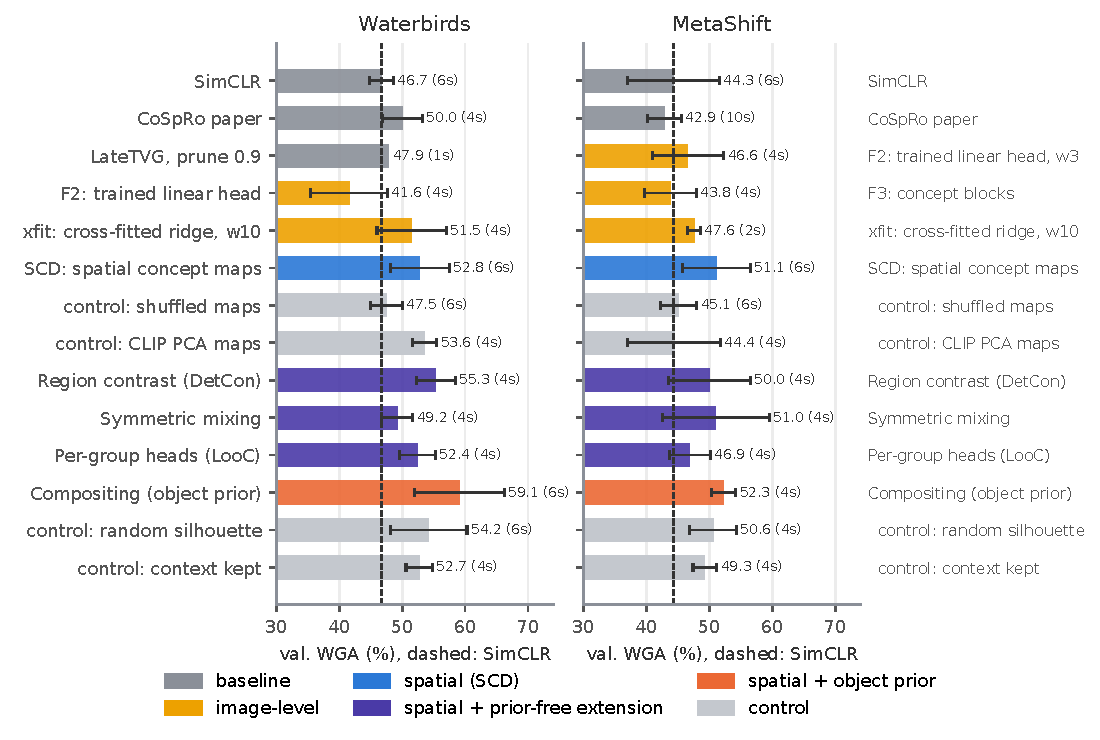
\includegraphics[width=\linewidth]{figures/scoreboard.pdf}
\caption{Every architecture of the branch on the two main datasets. Bars are validation WGA, whiskers one
standard deviation over seeds, ``(6s)'' the number of seeds. Grey bars are controls. The dashed line is
SimCLR. Section~\ref{sec:scoreboard} discusses this figure row by row.}
\label{fig:scoreboard}
\end{figure}

%=====================================================================
\section{Problem setting and baselines}
%=====================================================================

\subsection{Spurious correlations and worst-group accuracy}
Neural networks prefer the simplest feature that predicts the training labels, even when a harder feature
is the one that generalizes \citep{geirhos2020shortcut,shah2020simplicity}. In Waterbirds the bird type
agrees with the background on 95\% of the training images \citep{sagawa2020groupdro}. In MetaShift 88\% of
the training cats sit indoors and 88\% of the dogs outdoors \citep{liang2022metashift}. A representation that
learns ``water'' as evidence for ``waterbird'' or ``indoor'' as evidence for ``cat'' fails on the rare images
that break the rule. Each image belongs to a group $g=(y,a)$ of class $y$ and spurious attribute $a$. We
report average accuracy and the accuracy of the worst group \citep{sagawa2020groupdro}:
\begin{equation}
\mathrm{WGA}=\min_g \frac{1}{n_g}\sum_{i:\,g_i=g}\mathbf{1}\{\hat y_i=y_i\}.
\end{equation}

Self-supervised learning inherits these correlations from its unlabeled images. Contrastive objectives can
be met by the easiest discriminative feature and then suppress harder ones
\citep{chen2021intriguing,robinson2021shortcut}; easy features dominate the representation even when a
harder one is equally predictive \citep{hermann2020shapes}; image backgrounds alone carry much of the signal
that ImageNet models use \citep{xiao2021noise}.

\begin{table}[H]
\centering
\caption{Datasets. MetaShift and Spur-CIFAR10 served as development datasets; Waterbirds and CelebA
received frozen configurations.}
\small
\begin{tabularx}{\linewidth}{l r X}
\toprule
Dataset & Train images & Spurious structure and evaluation \\
\midrule
Waterbirds \citep{sagawa2020groupdro} & 4,795 & bird type vs.\ land/water background; validation groups 467 / 466 / 133 / 133 images, the two waterbird groups smallest; test 642 per minority group \\
MetaShift \citep{liang2022metashift} & 1,700 & cat/dog vs.\ indoor/outdoor, 88\% agreement; 72 validation images per group, so WGA is noisy (one image = 1.4 points) \\
Spur-CIFAR10 & 45,000 & CIFAR-10 classes \citep{krizhevsky2009cifar}; a 2-pixel coloured line agrees with the class on 95\% of the training images; 100 (class, colour) groups \\
CelebA \citep{liu2015celeba} & 162,770 & blond hair vs.\ gender; image-level runs only \\
\bottomrule
\end{tabularx}
\end{table}

\subsection{Why a linear probe on a balanced set suffices: deep feature reweighting}
Our evaluation fits a logistic regression on frozen features, the linear probe of representation analysis
\citep{alain2017probes}, using a small \emph{group-balanced} subset of
the training split (224 images on Waterbirds, 400 on MetaShift, 1,400 on Spur-CIFAR10). Deep feature
reweighting (DFR) showed that such a balanced last layer recovers high WGA whenever the representation
encodes the core feature apart from the spurious one \citep{kirichenko2023dfr}. \citet{izmailov2022feature}
showed further that WGA after last-layer retraining depends mainly on the quality of the representation,
and \citet{labonte2023lastlayer} that a few hundred balanced examples suffice for the retraining. The
quality of the representation is therefore the quantity to improve and the balanced probe measures it.

\paragraph{Goal derived from DFR.} The representation must contain a \emph{bird direction} and a
\emph{background direction} as two separate, linearly readable directions. It may keep the background; the
balanced probe then puts its weight on the bird direction. The failure to prevent is the \emph{fusion} of the
two into one direction (``waterbird-and-water'') or the \emph{suppression} of the harder feature by the easier
one (Figure~\ref{fig:fusion}).

\begin{figure}[H]
\centering
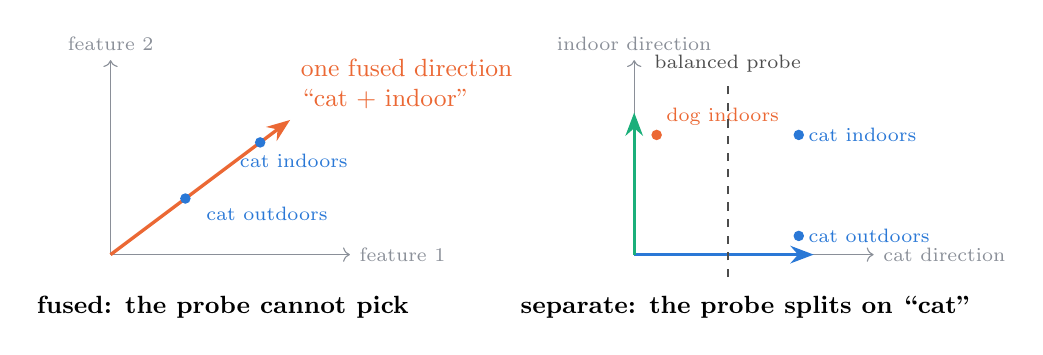
\begin{tikzpicture}[scale=0.95]
\begin{scope}
\draw[->,cgrey] (0,0)--(3.2,0) node[right,font=\scriptsize]{feature 1};
\draw[->,cgrey] (0,0)--(0,2.6) node[above,font=\scriptsize]{feature 2};
\draw[-{Stealth},very thick,corange] (0,0)--(2.4,1.8) node[above right,font=\small,align=left]{one fused direction\\``cat + indoor''};
\node[font=\small\bfseries] at (1.5,-0.7) {fused: the probe cannot pick};
\fill[cblue] (2.0,1.5) circle (2pt);
\fill[cblue] (1.0,0.75) circle (2pt);
\node[font=\scriptsize,cblue,anchor=west] at (1.15,0.55) {cat outdoors};
\node[font=\scriptsize,cblue] at (2.45,1.25) {cat indoors};
\end{scope}
\begin{scope}[xshift=7cm]
\draw[->,cgrey] (0,0)--(3.2,0) node[right,font=\scriptsize]{cat direction};
\draw[->,cgrey] (0,0)--(0,2.6) node[above,font=\scriptsize]{indoor direction};
\draw[-{Stealth},very thick,cblue] (0,0)--(2.4,0);
\draw[-{Stealth},very thick,cgreen] (0,0)--(0,1.9);
\fill[cblue] (2.2,1.6) circle (2pt) node[right,font=\scriptsize]{cat indoors};
\fill[cblue] (2.2,0.25) circle (2pt) node[right,font=\scriptsize]{cat outdoors};
\fill[corange] (0.3,1.6) circle (2pt) node[above right,font=\scriptsize]{dog indoors};
\draw[dashed,thick,black!70] (1.25,-0.3)--(1.25,2.3) node[above,font=\scriptsize]{balanced probe};
\node[font=\small\bfseries] at (1.5,-0.7) {separate: the probe splits on ``cat''};
\end{scope}
\end{tikzpicture}
\caption{The geometry behind the goal. Left: a fused direction places cats outdoors close to the origin,
so no linear probe separates them from dogs indoors. Right: with separate directions the balanced probe
uses the cat axis alone.}
\label{fig:fusion}
\end{figure}

\subsection{The restriction: no prior about which concept is spurious}
Label-free methods against spurious correlations rest on an assumption about what is spurious. LateTVG
\citep{hamidieh2024latetvg} and LA-SSL \citep{zhu2023lassl} assume that the spurious feature is the
\emph{easy} one, learned first or by the late layers. Background augmentation \citep{ryali2021background},
saliency-based copy-paste \citep{zhao2021dilo} and object-aware contrastive learning \citep{mo2021objectaware}
assume that it is the \emph{background}. CoSpRo assumed a \emph{removable context concept}. These assumptions
hold on some datasets and fail on others: in CelebA the spurious attribute (gender) is a property of the
person and lies in no background. The branch therefore adopts one restriction.

\paragraph{Restriction of the thesis method.} No step of pretraining uses target labels, group labels or
knowledge of which concept is the class and which the spurious attribute. Every concept enters the loss in
the same way. Labels enter only the balanced probe and the post-hoc analysis, identically for every method.

\subsection{What we compare against}
\begin{itemize}[leftmargin=*]
\item \textbf{SimCLR} \citep{chen2020simclr} under the identical protocol: the reference for every gain.
\item \textbf{A control for every new loss}: the same loss on another image's targets (``shuffled''). It
keeps every statistic of the targets and removes their link to the image content, so a gain above it is a
gain of the concept content. This follows the control tasks of the probing literature, which separate what
a representation encodes from what a flexible readout can fit \citep{hewitt2019control}. Most decisions of
the branch rest on these controls.
\item \textbf{CoSpRo} (our previous paper): \pmsd{50.64}{1.97} test WGA on Waterbirds against
\pmsd{46.82}{3.65} for SimCLR; on MetaShift \pmsd{42.9}{2.7} against \pmsd{44.6}{6.9} over ten seeds.
\item \textbf{LateTVG} \citep{hamidieh2024latetvg} reports 55.4 (Waterbirds) and 59.3 (MetaShift) WGA with
SimCLR under its own protocol. Under our protocol one seed reaches 47.9 on Waterbirds; the matched six-seed
test run is predeclared (\texttt{waterbirds\_latetvg\_test.yaml}).
\item \textbf{LA-SSL} \citep{zhu2023lassl} has an adaptation in the CoSpRo paper's appendix.
\end{itemize}
Absolute accuracies are low (SimCLR reaches 52\% average accuracy on Waterbirds) because a ResNet-18 trains
from random initialization on 1,700 to 4,795 images. Like LateTVG and LA-SSL, the protocol pretrains on the
dataset's own images and measures what the SSL objective learns from them. Numbers with ImageNet-pretrained
backbones (DFR reaches above 90\% WGA on Waterbirds with a pretrained ResNet-50) answer a different question.

%=====================================================================
\section{Starting point: CoSpRo}
%=====================================================================
CoSpRo removed the subspace of one concept group from the CLIP embeddings, kept image pairs that became
closer, filtered them (activation contrast, residual concept agreement, synthetic null groups) into a sparse
teacher graph and transferred the graph to a SimCLR student through graph-aware batches and a relational KL
loss in the spirit of relational distillation \citep{park2019rkd}. On Waterbirds it gained about four points
of test WGA.

Two observations ended this line. First, the gain stayed on Waterbirds: CoSpRo scored below SimCLR on
MetaShift over ten seeds and 19.6 against 15.6 on one Spur-CIFAR10 seed. Second, the method carries the prior
that the spurious attribute is a removable context concept, the graph keeps wrong-class edges and the
background stays linearly decodable at 91\%.

%=====================================================================
\section{Shared components of every architecture}
%=====================================================================

\subsection{Training and evaluation protocol}
\begin{table}[H]
\centering
\caption{Protocol shared by every run of the branch (inherited from CoSpRo so that numbers are comparable).}
\small
\begin{tabularx}{\linewidth}{l X}
\toprule
Student & ResNet-18 \citep{he2016resnet} from random initialization. Waterbirds, MetaShift, CelebA: 224-pixel input (``large'' stem, $7\times7$ convolution with stride 2 and max-pooling). Spur-CIFAR10: 32-pixel input (CIFAR stem) \\
SSL & SimCLR \citep{chen2020simclr}, 500 epochs (CelebA 250), batch 128, temperature 0.05, SGD with learning rate 0.01 decayed by 0.1 at epochs 350, 400 and 450, weight decay $10^{-4}$, crop scale $[0.2,1]$, float16 autocast with a GradScaler \citep{micikevicius2018mixed} on one V100 \\
Probe & logistic regression (L2 coefficient 0.001) on the pooled 512-d features, fitted on the group-balanced subset of the training split, evaluated every 25 epochs \\
Reported value & mean of the last four probes (epochs 425 to 500); this damps single-probe noise on MetaShift's 72-image groups \\
Seeds & 4 to 6 for Waterbirds and MetaShift, 2 for Spur-CIFAR10 and CelebA; differences are reported paired by seed \citep{bouthillier2021variance} \\
Split & validation; the locked test split stays unused until the configuration is final \citep{gulrajani2021lost} \\
\bottomrule
\end{tabularx}
\end{table}

\subsection{The ResNet-18 student and why the concept loss reads the $7\times7$ map}
\label{sec:resnet}
\begin{figure}[H]
\centering
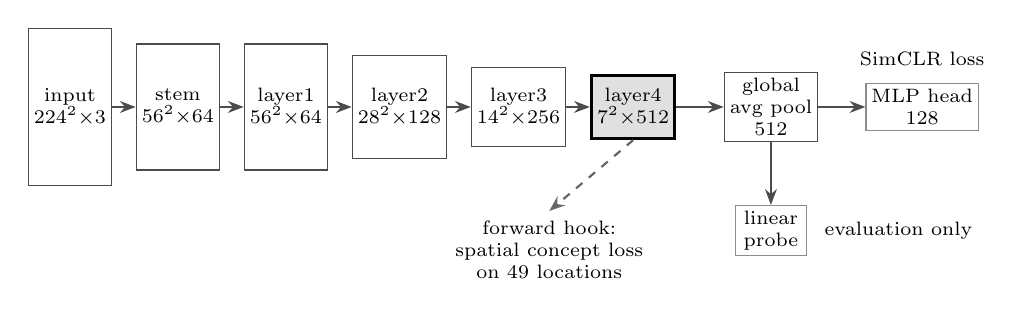
\begin{tikzpicture}[node distance=3mm,
 l/.style={draw=black!70,fill=white,minimum width=9mm,align=center,font=\scriptsize,inner sep=2pt}]
\node[l,minimum height=20mm] (in) {input\\$224^2{\times}3$};
\node[l,minimum height=16mm,right=of in] (c1) {stem\\$56^2{\times}64$};
\node[l,minimum height=16mm,right=of c1] (l1) {layer1\\$56^2{\times}64$};
\node[l,minimum height=13mm,right=of l1] (l2) {layer2\\$28^2{\times}128$};
\node[l,minimum height=10mm,right=of l2] (l3) {layer3\\$14^2{\times}256$};
\node[l,minimum height=8mm,right=of l3,fill=black!12,draw=black,very thick] (l4) {layer4\\$7^2{\times}512$};
\node[l,minimum height=6mm,right=6mm of l4] (gap) {global\\avg pool\\512};
\node[l,minimum height=6mm,right=6mm of gap,draw=black!45] (head) {MLP head\\128};
\node[l,minimum height=6mm,below=8mm of gap,draw=black!45] (probe) {linear\\probe};
\draw[arr] (in)--(c1); \draw[arr] (c1)--(l1); \draw[arr] (l1)--(l2); \draw[arr] (l2)--(l3); \draw[arr] (l3)--(l4);
\draw[arr] (l4)--(gap); \draw[arr] (gap)--(head); \draw[arr] (gap)--(probe);
\node[above=1mm of head,font=\scriptsize,align=center] {SimCLR loss};
\node[below left=9mm and -8mm of l4,font=\scriptsize,align=center] (hook) {forward hook:\\spatial concept loss\\on 49 locations};
\draw[darr] (l4.south)--(hook.north);
\node[right=1mm of probe,font=\scriptsize] {evaluation only};
\end{tikzpicture}
\caption{The student. SimCLR and the probe read the 512-d vector after global average pooling. The
spatial concept loss reads the $7\times7\times512$ output of \texttt{layer4} through a forward hook,
\emph{before} pooling. Spur-CIFAR10 uses the CIFAR stem, so its map is $4\times4\times512$.}
\label{fig:resnet}
\end{figure}

The network keeps every layer; the spatial loss taps the tensor that global average pooling would average.
Four reasons fix this choice.
\begin{itemize}[leftmargin=*]
\item \textbf{Pooling is where concepts fuse.} Global average pooling \citep{lin2014nin} turns the map into
one 512-d vector per image, so a cat and a couch in the same image become one vector. Across images they
co-occur (88\%) and an image-level target separates ``cat'' from ``couch'' only on the few images where they
disagree. In the $7\times7$ map they occupy different locations of \emph{every} image. Class activation maps
rest on the same property: the last convolutional map before pooling still localizes the objects that the
pooled vector mixes \citep{zhou2016cam}.
\item \textbf{The last stage carries object and scene semantics and feeds the probe.} Units of the last
convolutional stage respond to objects and scenes, earlier stages to textures and parts
\citep{bau2017dissection}. \texttt{layer4} feeds the pooled vector directly, so shaping it shapes exactly the
representation the probe evaluates. Regressing a teacher signal from an intermediate feature map through a
small readout is the hint training of FitNets \citep{romero2015fitnets}; dense SSL methods attach their losses
to the same map \citep{wang2021densecl,xie2021pixpro,henaff2021detcon}.
\item \textbf{$7=224/32$.} ResNet-18 halves the resolution five times (stem convolution, max-pooling,
\texttt{layer2}, \texttt{layer3}, \texttt{layer4}); 49 locations remain.
\item \textbf{A limitation built into this choice.} The theoretical receptive field of a \texttt{layer4} unit
exceeds the 224-pixel view \citep{araujo2019receptive}; the effective receptive field is a smaller central
region that still spans a large part of the view \citep{luo2016erf}. A ``cat'' location therefore also sees
the scene, which is why the student keeps part of the co-occurrence (Section~\ref{sec:audit}).
\end{itemize}

\subsection{SpLiCE concepts}
\label{sec:splice}
A frozen OpenCLIP ViT-B/32 (LAION-2B weights; \citealp{radford2021clip}) embeds every training image as $z_i$.
SpLiCE \citep{bhalla2024splice} writes the centred, normalized embedding as a sparse non-negative combination
of text directions from a vocabulary,
\begin{equation}
u_i=\operatorname{norm}(z_i-\mu),\qquad c_i\in\arg\min_{c\ge0}\|u_i-D^\top c\|_2^2+\lambda_1\|c\|_1,
\end{equation}
with L1 penalty 0.25. About nine concepts are active per image. MetaShift uses the LAION vocabulary (10,000
words), Waterbirds and Spur-CIFAR10 the Open Images v7 vocabulary (20,931 words). SpLiCE supplies a vocabulary
of the concepts that occur in the training set, named and found without labels.

\subsection{From concepts to concept factors: the meaning grouping}
\label{sec:grouping}
\summary A vocabulary names one visual content several times (\emph{cat, kitten, kitty}). A \emph{concept
factor} is a group of concepts that name one thing; its value on an image is the sum of its members' SpLiCE
codes. The CoSpRo grouping rule, which required co-activation, left almost every concept alone and chained a
bird to its background when its thresholds were lowered. The meaning grouping clusters concepts by raw CLIP
text similarity with average linkage and a response veto. It works: it joins synonyms and keeps an object
apart from its context on every dataset, because raw text embeddings place synonyms far closer than
object--context pairs (Figure~\ref{fig:signals}).

\begin{figure}[H]
\centering
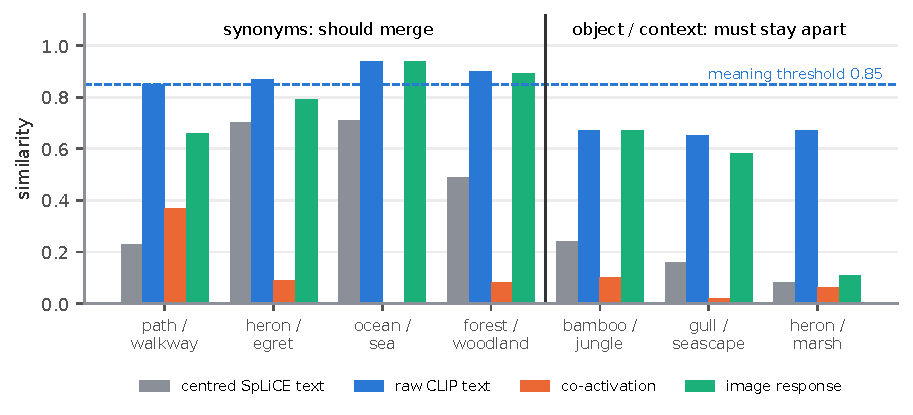
\includegraphics[width=0.95\linewidth]{figures/grouping_signals.pdf}
\caption{Four similarity signals on Waterbirds concept pairs. Co-activation (orange) fails for synonyms:
the L1 penalty activates one of two synonyms per image (heron and egret co-activate at 0.09, ocean and sea at
0.00). Centred SpLiCE text directions (grey) also separate synonyms. Raw CLIP text embeddings (blue) put
synonyms at 0.85 to 0.94 and object--context pairs at 0.64 to 0.72, so a threshold at 0.85 separates them.}
\label{fig:signals}
\end{figure}

\paragraph{Why co-activation fails.} The L1 penalty of the lasso selects one variable out of a group of
strongly correlated ones and sets the others to zero \citep{tibshirani1996lasso,zou2005elasticnet}. SpLiCE
inherits this behaviour: two synonyms are near-duplicate dictionary rows, so each image activates one of them.
On Waterbirds 499 of 502 CoSpRo groups were single concepts. Lowering both thresholds linked concepts through
chains of pairwise matches, the known failure of single linkage, which is what connected components of a
pairwise graph compute \citep{murtagh2012hierarchical}: one group held hummingbird, parrot, jungle and bamboo.

\paragraph{The procedure} (\texttt{cospro/cli/build\_meaning\_groups.py}):
\begin{enumerate}[leftmargin=*]
\item keep concepts active on 0.2\% to 95\% of the training images;
\item similarity $s_{k\ell}=\cos(t_k,t_\ell)$ of the raw CLIP text embeddings, set to $-1$ (veto) when the
images' responses $u_i^\top d_k$ and $u_i^\top d_\ell$ correlate below 0.5;
\item average-linkage clustering cut at text similarity 0.85. Average linkage joins two clusters only when
their members agree on average, which stops chains \citep{murtagh2012hierarchical};
\item a factor's text direction is the normalized mean of its members' text embeddings;
\item keep factors active on 2\% to 90\% of the images (5\% to 90\% for the image-level variants).
\end{enumerate}
Examples: \{kitty, kitten, cat\}, \{canine, dog\}, \{cozy, comfy, cosy\}. Result: 242 factors on Waterbirds, 130 on
MetaShift and 147 on Spur-CIFAR10 (2\% band).

\paragraph{Why these numbers.}
\begin{itemize}[leftmargin=*]
\item \textbf{Text similarity 0.85} lies between synonyms (0.85--0.94) and object--context pairs (0.64--0.72); a
sweep over 576 factor sets on MetaShift chose it together with the response veto 0.5.
\item \textbf{Response veto 0.5}: two words with similar text whose images respond differently stay apart
(heron and marsh: response correlation 0.11).
\item \textbf{Frequency band 2\%--90\%}: a factor on fewer than 2\% of the images occurs about once per
half batch (64 images), so a fit on half a batch cannot learn it. At 5\% the MetaShift factors lose every
scene concept (couch, lawn, bed, window, bench); at 2\% they keep them. Factors above 90\% carry no contrast
between images.
\end{itemize}

%=====================================================================
\section{Overview of the explored architectures}
%=====================================================================
The architectures form three lines of work. Each line answers a question raised by the previous one:
image-level targets show that concepts help and that small datasets are memorized; spatial targets remove the
memorization and raise WGA on every dataset; the third line tries to separate the object from its usual
context, which the spatial student leaves fused.

\begin{figure}[H]
\centering
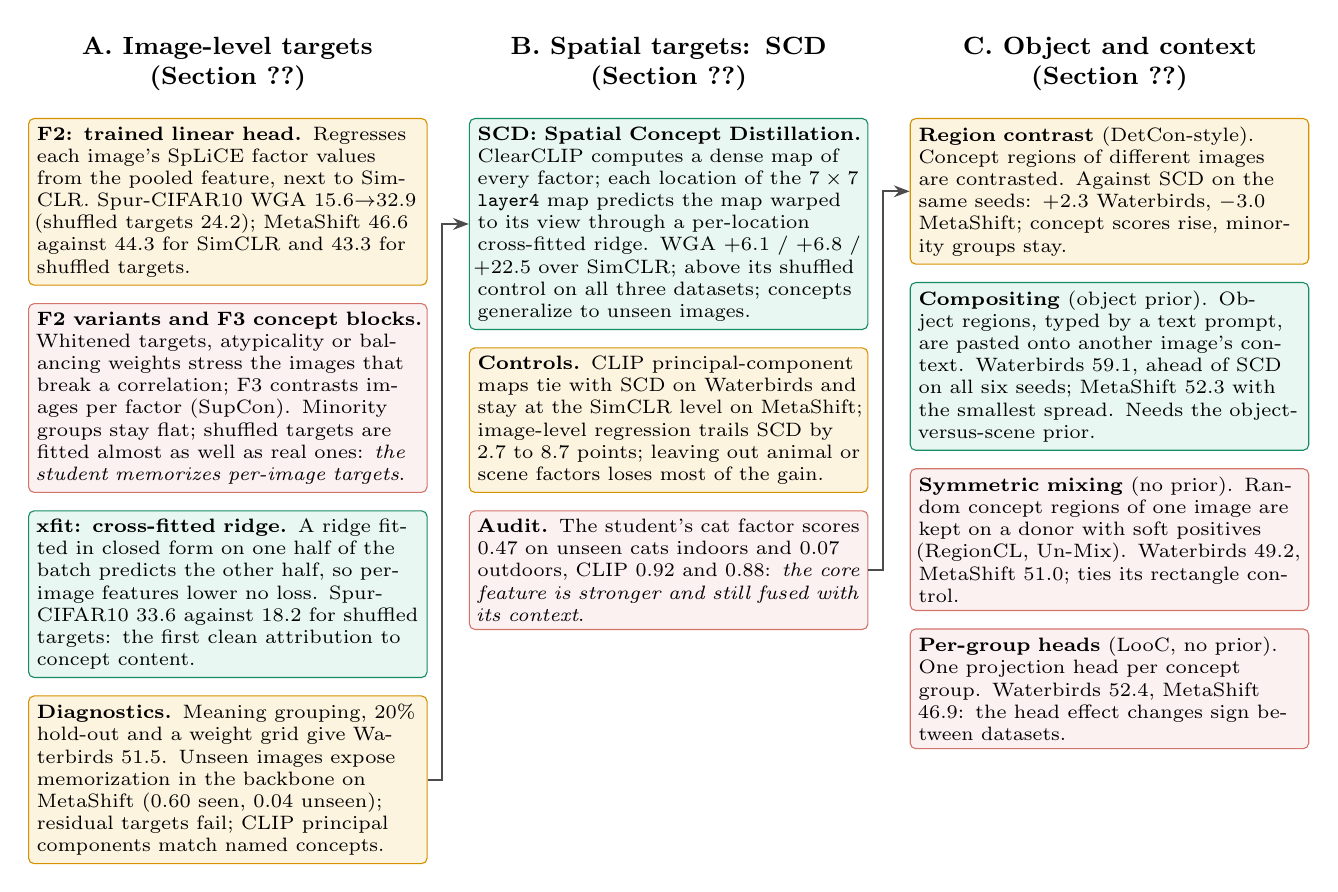
\begin{tikzpicture}[node distance=2.2mm,
  st/.style={draw,rounded corners=2pt,align=left,font=\scriptsize,text width=48.5mm,inner sep=3pt},
  ok/.style={st,fill=cgreen!10,draw=cgreen!80!black},
  no/.style={st,fill=cred!7,draw=cred!70},
  mx/.style={st,fill=cyellow!12,draw=cyellow!90!black},
  ph/.style={font=\small\bfseries,align=center,text width=48.5mm}]
% Line A
\node[ph] (pa) {A. Image-level targets\\(Section~\ref{sec:imagelevel})};
\node[mx,below=of pa] (a2) {\textbf{F2: trained linear head.} Regresses each image's SpLiCE factor values from the pooled feature, next to SimCLR. Spur-CIFAR10 WGA 15.6$\to$32.9 (shuffled targets 24.2); MetaShift 46.6 against 44.3 for SimCLR and 43.3 for shuffled targets.};
\node[no,below=of a2] (a3) {\textbf{F2 variants and F3 concept blocks.} Whitened targets, atypicality or balancing weights stress the images that break a correlation; F3 contrasts images per factor (SupCon). Minority groups stay flat; shuffled targets are fitted almost as well as real ones: \emph{the student memorizes per-image targets}.};
\node[ok,below=of a3] (a4) {\textbf{xfit: cross-fitted ridge.} A ridge fitted in closed form on one half of the batch predicts the other half, so per-image features lower no loss. Spur-CIFAR10 33.6 against 18.2 for shuffled targets: the first clean attribution to concept content.};
\node[mx,below=of a4] (a5) {\textbf{Diagnostics.} Meaning grouping, 20\% hold-out and a weight grid give Waterbirds 51.5. Unseen images expose memorization in the backbone on MetaShift (0.60 seen, 0.04 unseen); residual targets fail; CLIP principal components match named concepts.};
% Line B
\node[ph,right=5mm of pa] (pb) {B. Spatial targets: SCD\\(Section~\ref{sec:scd})};
\node[ok,below=of pb] (b1) {\textbf{SCD: Spatial Concept Distillation.} ClearCLIP computes a dense map of every factor; each location of the $7\times7$ \texttt{layer4} map predicts the map warped to its view through a per-location cross-fitted ridge. WGA $+6.1$ / $+6.8$ / $+22.5$ over SimCLR; above its shuffled control on all three datasets; concepts generalize to unseen images.};
\node[mx,below=of b1] (b2) {\textbf{Controls.} CLIP principal-component maps tie with SCD on Waterbirds and stay at the SimCLR level on MetaShift; image-level regression trails SCD by 2.7 to 8.7 points; leaving out animal or scene factors loses most of the gain.};
\node[no,below=of b2] (b3) {\textbf{Audit.} The student's cat factor scores 0.47 on unseen cats indoors and 0.07 outdoors, CLIP 0.92 and 0.88: \emph{the core feature is stronger and still fused with its context}.};
% Line C
\node[ph,right=5mm of pb] (pc) {C. Object and context\\(Section~\ref{sec:objectcontext})};
\node[mx,below=of pc] (c1) {\textbf{Region contrast} (DetCon-style). Concept regions of different images are contrasted. Against SCD on the same seeds: $+2.3$ Waterbirds, $-3.0$ MetaShift; concept scores rise, minority groups stay.};
\node[ok,below=of c1] (c2) {\textbf{Compositing} (object prior). Object regions, typed by a text prompt, are pasted onto another image's context. Waterbirds 59.1, ahead of SCD on all six seeds; MetaShift 52.3 with the smallest spread. Needs the object-versus-scene prior.};
\node[no,below=of c2] (c3) {\textbf{Symmetric mixing} (no prior). Random concept regions of one image are kept on a donor with soft positives (RegionCL, Un-Mix). Waterbirds 49.2, MetaShift 51.0; ties its rectangle control.};
\node[no,below=of c3] (c4) {\textbf{Per-group heads} (LooC, no prior). One projection head per concept group. Waterbirds 52.4, MetaShift 46.9: the head effect changes sign between datasets.};
\draw[arr] (a5.east) -- ++(1.8mm,0) |- (b1.west);
\draw[arr] (b3.east) -- ++(1.8mm,0) |- (c1.west);
\end{tikzpicture}
\caption{Map of the explored architectures. Green: kept; yellow: partial or informative; red: below the
reference or explained away by a control. Numbers are validation WGA.}
\label{fig:roadmap}
\end{figure}

%=====================================================================
\section{Image-level concept distillation}
\label{sec:imagelevel}
%=====================================================================
The methods of this section attach the concept targets to whole images: every image receives one vector of
factor values, which the student predicts from its pooled feature. This is the simplest form of distilling a
teacher's concepts \citep{hinton2015distilling} and the natural first test of the goal of
Section~\ref{sec:grouping}.

\subsection{F2: factor distillation with a trained linear head}
\summary A linear head on the pooled feature regresses each image's SpLiCE factor values next to the SimCLR
loss. It doubles WGA on Spur-CIFAR10 (15.6 to 32.9) and leaves MetaShift within the seed noise of SimCLR, with
the gain in the majority groups. Reweighting and whitening variants change little. The cause is memorization:
on 1,700 images the trained head fits shuffled targets almost as well as real ones, so the loss is met without
learning concepts.

\begin{figure}[H]
\centering
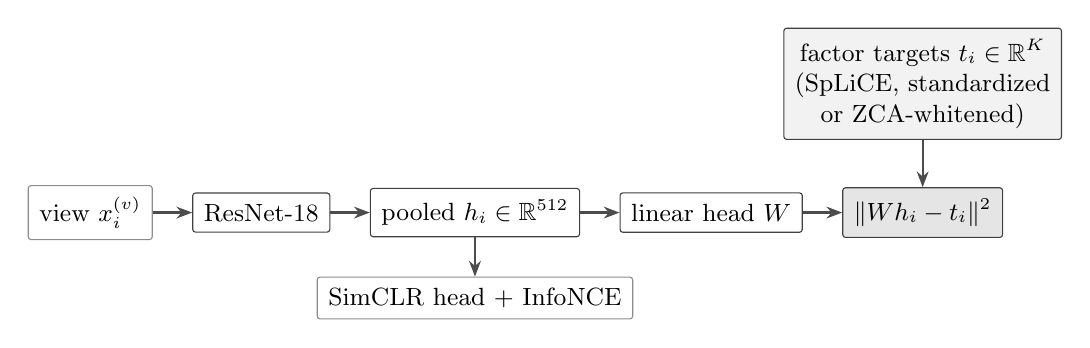
\begin{tikzpicture}[node distance=5mm]
\node[gbox] (img) {view $x_i^{(v)}$};
\node[sbox,right=of img] (enc) {ResNet-18};
\node[sbox,right=of enc] (h) {pooled $h_i\in\mathbb{R}^{512}$};
\node[sbox,right=of h] (W) {linear head $W$};
\node[lbox,right=of W] (L) {$\lVert W h_i - t_i\rVert^2$};
\node[tbox,above=6mm of L] (t) {factor targets $t_i\in\mathbb{R}^K$\\(SpLiCE, standardized\\or ZCA-whitened)};
\node[gbox,below=5mm of h] (simclr) {SimCLR head + InfoNCE};
\draw[arr] (img)--(enc); \draw[arr] (enc)--(h); \draw[arr] (h)--(W); \draw[arr] (W)--(L); \draw[arr] (t)--(L);
\draw[arr] (h)--(simclr);
\end{tikzpicture}
\caption{F2. A linear head predicts each image's factor values from the pooled backbone feature. The head is
linear so that the factors must be linearly readable, as the probe reads them.}
\end{figure}
The loss is $\mathcal L=\mathcal L_{\text{SimCLR}}+\lambda\,\frac{1}{2B}\sum_{i,v}\lVert W h_i^{(v)}-t_i\rVert^2/K$,
with the weight $\lambda$ switched on at epoch 10 after a 10-epoch linear warm-up. Three variants target the
images that break a correlation:
\begin{itemize}[leftmargin=*]
\item \textbf{Whitened targets} (ZCA, ridge 0.1; \citealp{kessy2018whitening}) keep for each factor the part the
other factors leave unexplained. This part is large exactly on the images that break a correlation.
\item \textbf{Atypicality weights} scale each image's loss by its mean squared whitened factor value: images
whose concepts break the dataset's correlations receive more weight (minority images about twice the weight on
a synthetic fixture). The idea is the upweighting of hard examples in JTT \citep{liu2021jtt}, computed from
concepts.
\item \textbf{Balancing weights} are per-image weights that minimize the squared correlations between factor
presences, so that under them ``indoor'' no longer predicts ``cat''. This is the sample reweighting of stable
learning \citep{shen2020stable,zhang2021deepstable}.
\end{itemize}

\begin{table}[H]
\centering
\caption{F2 results (validation WGA / average accuracy; groups on MetaShift: cat-in / cat-out / dog-in / dog-out).}
\small
\begin{tabular}{llccc}
\toprule
Dataset & Arm & WGA & Acc. & Groups \\
\midrule
Spur-CIFAR10 & SimCLR & \pmsd{15.6}{1.0} & 59.5 & \\
 & F2, standardized & \pmsd{32.9}{1.6} & 69.5 & \\
 & F2, shuffled targets & \pmsd{24.2}{0.4} & 58.6 & \\
\midrule
MetaShift & SimCLR & \pmsd{44.3}{7.3} & 55.2 & 57 / 47 / 53 / 64 \\
 & F2, weight 3 & \pmsd{46.6}{5.7} & 61.5 & 70 / 47 / 54 / 74 \\
 & F2, weight 3, shuffled & \pmsd{43.3}{8.1} & 54.8 & 57 / 45 / 53 / 65 \\
 & F2, whitened, weight 3 & \pmsd{47.9}{6.4} & 56.9 & 57 / 51 / 55 / 65 \\
 & F2, atypicality weights & \pmsd{50.5}{3.8} & 58.8 & 59 / 52 / 55 / 70 \\
 & F2, balancing weights & \pmsd{44.2}{8.1} & 59.0 & 64 / 44 / 55 / 72 \\
\midrule
Waterbirds & F2 (first frozen configuration) & \pmsd{41.6}{6.1} & 51.2 & below SimCLR \\
\bottomrule
\end{tabular}
\end{table}

\begin{figure}[H]
\centering
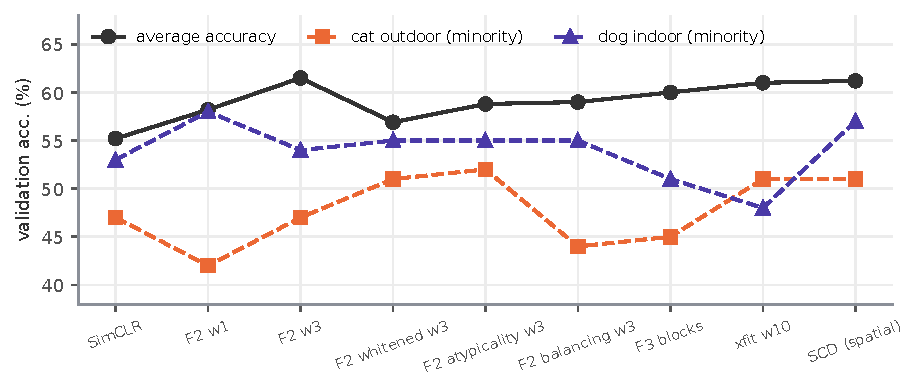
\includegraphics[width=0.92\linewidth]{figures/metashift_rounds.pdf}
\caption{MetaShift across the image-level variants. Average accuracy rises with almost every concept loss;
the two minority groups (cat outdoors, dog indoors) stay within a few points of SimCLR. The gain goes to
the majority groups.}
\label{fig:rounds}
\end{figure}

\subsection{F3: concept blocks (supervised contrast per factor)}
\summary One small embedding block per factor applies a supervised contrastive loss in which two images that
both show the factor are positives, weighted towards pairs whose other concepts differ. The idea is that a
fused ``cat-and-indoor'' direction cannot rank ``cat on street'' above ``dog on sofa'' inside the cat block. On
MetaShift it scores 43.8 WGA, below its own controls and the loss reaches the same value with shuffled
concepts: the blocks are met by memorization as well.

\textbf{Method.} The 32 most balanced factors each get a linear block. Inside block $k$, images that both show
factor $k$ are positives under SupCon \citep{khosla2020supcon}; a positive pair weighs more when the two images'
other factors differ (``cat on sofa'' with ``cat on street''). The backbone would then need a cat direction that
survives a change of context. \textbf{Result:} \pmsd{43.8}{4.1} WGA; the control with uniform pair weights scored
\pmsd{49.7}{2.5} and the shuffled control \pmsd{46.4}{3.5}.

\subsection{Diagnosis: the student memorizes per-image targets}
The controls explain every MetaShift result. F2 at weight 3 explains 0.41 of the real target variance and 0.33
of the shuffled one; the F3 block loss ends at 3.34 with real concepts and 3.37 with shuffled ones. Deep networks
fit random labels on small datasets \citep{zhang2017rethinking,arpit2017memorization} and a SimCLR backbone is
built to tell individual images apart \citep{wu2018instance,wang2020alignment}. A per-image target on 1,700
images can therefore be read off the instance identity that SimCLR provides anyway. Any auxiliary loss attached
to single images is then met without learning concepts. On Spur-CIFAR10 (45,000 images) shuffled targets reach
only 0.02 explained variance, so the concepts shape the student there. The remedy has to remove the reward for
memorizing an image; the cross-fit of the next section does exactly that.

\subsection{xfit: the cross-fitted ridge}
\label{sec:xfit}
\summary The trained head is replaced by a ridge regression fitted in closed form on one half of the batch and
evaluated on the other half. A feature that only identifies one image carries nothing to the other half, so
memorization lowers no part of the loss. On Spur-CIFAR10 xfit matches F2 (33.6 WGA) while its shuffled control
falls to the SimCLR level: the whole gain comes from the concept content. On MetaShift it removes the
memorization of the head and leaves WGA at the SimCLR level, because the backbone still stores the targets of
its training images (Section~\ref{sec:holdout}).

\textbf{Idea.} Fitting an auxiliary model on one part of the sample and evaluating it on another is the
sample splitting (cross-fitting) of double machine learning \citep{chernozhukov2018dml}. We apply it to a training loss: only
directions that transfer from half $A$ to half $B$ lower the error. The ridge is solved in closed form and
differentiated through, as in the closed-form heads of R2D2 \citep{bertinetto2019r2d2} and MetaOptNet
\citep{lee2019metaoptnet}, so the backbone receives gradients through the solve.

\begin{figure}[H]
\centering
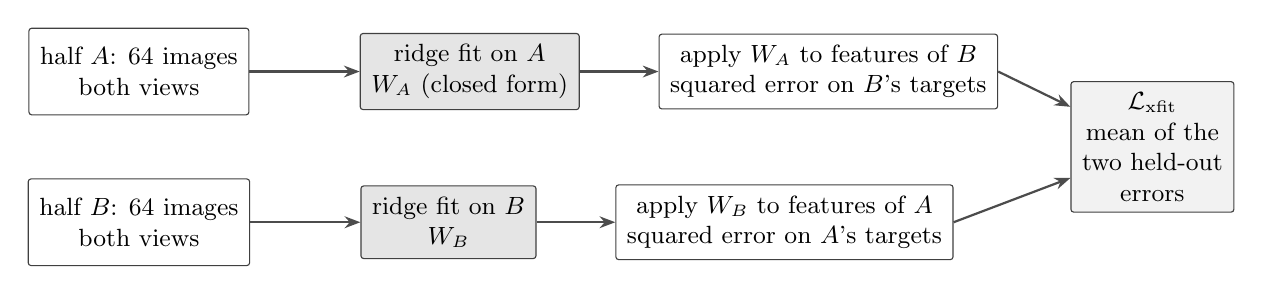
\begin{tikzpicture}[node distance=4mm]
\node[sbox,minimum width=26mm,minimum height=11mm] (A) {half $A$: 64 images\\both views};
\node[sbox,minimum width=26mm,minimum height=11mm,below=8mm of A] (B) {half $B$: 64 images\\both views};
\node[lbox,right=14mm of A] (fitA) {ridge fit on $A$\\$W_A$ (closed form)};
\node[lbox,right=14mm of B] (fitB) {ridge fit on $B$\\$W_B$};
\node[box,right=10mm of fitA] (predB) {apply $W_A$ to features of $B$\\squared error on $B$'s targets};
\node[box,right=10mm of fitB] (predA) {apply $W_B$ to features of $A$\\squared error on $A$'s targets};
\node[tbox,right=12mm of $(predB.east)!0.5!(predA.east)$] (loss) {$\mathcal L_{\text{xfit}}$\\mean of the\\two held-out\\errors};
\draw[arr] (A)--(fitA); \draw[arr] (B)--(fitB);
\draw[arr] (fitA)--(predB); \draw[arr] (fitB)--(predA);
\draw[arr] (predB.east)--(loss); \draw[arr] (predA.east)--(loss);
\end{tikzpicture}
\caption{Cross-fitting. Gradients flow through the solve and the prediction into the backbone. Both views
of an image stay in the same half, so no half sees a view of an image it predicts.}
\label{fig:xfit}
\end{figure}

With unit-norm centred features $H$, targets $T$ and per-image weights $D$, the dual (kernel) form of the ridge
\citep{hoerl1970ridge,saunders1998dual} is
\begin{equation}
\hat T_B = H_B H_A^\top\big(D_A H_A H_A^\top+\rho I\big)^{-1} D_A T_A,
\end{equation}
one $n\times n$ solve per half (code: \texttt{cross\_fit\_predictions} in
\texttt{cospro/methods/concept\_factors.py}).

\paragraph{Why unit-norm rows and an absolute ridge $\rho=1$.} The first version scaled the ridge with the
feature norm, which made it small. Fits of 64 images in 512 dimensions then nearly interpolated, the solve became
ill conditioned, three of four Spur-CIFAR10 runs produced NaN features and the held-out explained variance was
negative everywhere. Normalizing every feature row stops the backbone from weakening the ridge by shrinking its
features and an absolute ridge keeps every eigenvalue of the system at least $\rho$ \citep{hoerl1970ridge}.
Ridge 10 performed no better on MetaShift (42.5 WGA).

\begin{table}[H]
\centering
\caption{Cross-fit with unit-norm rows and $\rho=1$ (seeds 1 and 2). Batch EV: held-out explained variance of the
in-batch fit.}
\small
\begin{tabular}{llccc}
\toprule
Dataset & Arm & WGA & Acc. & Batch EV \\
\midrule
Spur-CIFAR10 & SimCLR & \pmsd{15.6}{1.0} & 59.5 & \\
 & F2 trained head & \pmsd{32.9}{1.6} & 69.5 & 0.10 \\
 & \textbf{xfit} & \pmsd{33.6}{2.3} & 69.7 & 0.13 \\
 & xfit, shuffled & \pmsd{18.2}{3.2} & 57.5 & $-0.02$ \\
\midrule
MetaShift & xfit (145 factors) & \pmsd{43.9}{3.2} & 54.8 & $-0.01$ \\
 & xfit, shuffled & \pmsd{41.7}{0.0} & 54.4 & $-0.03$ \\
\bottomrule
\end{tabular}
\end{table}

\subsection{What the student can learn: bounds, weights and unseen images}
\label{sec:holdout}
\textbf{Learnability bound.} A ridge fitted on 64 images can only predict factors that occur often enough.
Running the same fit on frozen CLIP features gives an upper bound: with 278 factors from 1\% frequency even CLIP
scores $-0.015$; with the 24 factors from 5\% it scores 0.16 (shuffled: $-0.07$). Hence the 5\% band for
image-level runs.

\textbf{Loss weight.} At weight 10 the 24 MetaShift factors reach 0.72 to 0.87 explained variance on the
training images, \emph{three times the CLIP score}, while WGA stays at 45.5. A probe on the 24 factor values
themselves reaches 77\% WGA. The student stores something other than the concepts.

\textbf{The hold-out diagnostic.} A fixed fifth of the training images gets loss weight 0 in the concept loss
(SimCLR still trains on them). A ridge fitted on the other images then scores the factors on these \emph{unseen}
images. This exposes memorization in the backbone, which the cross-fit cannot see: the cross-fit removes the
reward for memorizing inside one batch, while the backbone can still store each training image's targets across
epochs.

\begin{figure}[H]
\centering
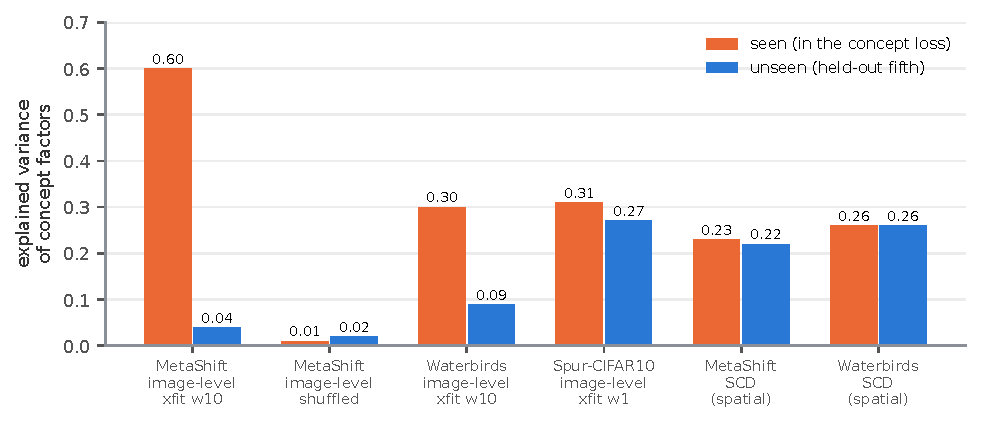
\includegraphics[width=0.95\linewidth]{figures/memorization.pdf}
\caption{Explained variance of the factors on images inside the concept loss (seen) and outside it (unseen).
Image-level xfit on MetaShift: 0.60 seen, 0.04 unseen; the backbone stores the targets of its 1,700 images.
Spur-CIFAR10 (45,000 images) generalizes: 0.31 against 0.27. SCD (spatial, scored on dense responses)
shows no gap on either dataset.}
\label{fig:memorization}
\end{figure}

\subsection{Waterbirds with the frozen image-level configuration}
The configuration chosen on MetaShift (meaning factors from 5\%, 70 Open Images factors, weight 10, hold-out)
reaches 55.3 WGA on the first two Waterbirds seeds and \pmsd{51.5}{5.5} on four, with accuracy 57.5 against 52.3
for SimCLR and \pmsd{41.4}{3.0} for its shuffled control. The same configuration on Spur-CIFAR10 drops to 22.7
(weight 1 gives 33.6): at weight 10 even 45,000 images are memorized. The weight grid on Spur-CIFAR10 shows that
the unseen score cannot choose the weight label-free (0.32 to 0.33 for weights 1 to 10 while WGA moves within
noise).

\subsection{Two final diagnostics}
\textbf{Decoupling score.} Each factor minus its linear regression on the other factors (its \emph{residual}) is
the part a fused direction cannot predict. The student explains 0.03 to 0.04 of the residuals against 0.15 to
0.17 for CLIP. Training directly on residual targets fails: the student cannot predict them and Waterbirds WGA
falls to \pmsd{41.7}{0.9}, the level of the shuffled control.

\textbf{CLIP control.} Distilling as many principal components of the CLIP image embeddings as there are factors
gives the same or better numbers (Waterbirds 51.0, MetaShift 54.2, Spur-CIFAR10 36.3 to 37.0). At the image level
the concept names add nothing over generic CLIP information, in line with plain feature distillation from CLIP
\citep{yang2024clipkd}.

\subsection{Outcome of the image-level line}
Image-level concept distillation helps when the student can generalize the targets (Spur-CIFAR10: 15.6 to 33.6;
Waterbirds: 46.7 to 51.5) and the cross-fit makes the attribution clean. Three findings limit it: small
datasets are memorized in the backbone; the student learns the part the factors share, which is the dataset's
co-occurrence \citep{trauble2021correlated}; named concepts match CLIP principal components. Image-level targets
can separate ``cat'' from ``couch'' only through the images where the two disagree. That limit motivated the
spatial loss.

%=====================================================================
\section{Spatial Concept Distillation (SCD)}
\label{sec:scd}
%=====================================================================
\summary SCD tells the student \emph{where} each concept is. A frozen CLIP model computes a dense map of every
concept factor over every training image; during SimCLR training every location of the student's $7\times7$
feature map predicts the concept values at its place in the view, through the cross-fitted ridge of
Section~\ref{sec:xfit}. SCD works: it is the first method of the project that beats its shuffled control on every
dataset tested (WGA $+6.1$, $+6.8$ and $+22.5$ over SimCLR on Waterbirds, MetaShift and Spur-CIFAR10) and its
concepts generalize to images outside the loss. It works because location separates concepts that co-occur in
images: cat and couch share an image label but occupy different cells, so the student must encode both. Its
limit is that each cell sees most of the view, so the student still predicts the cat partly from the scene.
SCD is the prior-free method of the thesis; this section describes it in the form of the paper draft
(\texttt{paper/SpatialConcepts.tex}).

\subsection{Motivation}
SSL representations inherit the co-occurrences of their unlabeled training images: when cats appear mostly
indoors, an encoder trained from scratch learns indoor scenes as evidence for cats. Deep feature reweighting shows
that a linear head retrained on a small group-balanced set recovers WGA whenever the representation encodes the
core feature apart from the spurious one \citep{kirichenko2023dfr}. A frozen vision-language model supplies semantic
structure learned from external data and SpLiCE exposes it as sparse non-negative coordinates associated with text
concepts \citep{bhalla2024splice}. The image-level experiments show that these coordinates help when the student
can generalize them and fail where the concepts co-occur. We hypothesize that the \emph{location} of a concept is
the missing signal: at the image level cat and couch appear together, while at the pixel level they occupy
different places in every image.

\subsection{Related work}
\paragraph{Dense and region-level self-supervised learning.} SimCLR contrasts two views of an image against the other
images in the batch \citep{chen2020simclr} and pools the feature map before its projection head. VADeR and DenseCL
add a contrastive loss between matched locations of the two views \citep{pinheiro2020vader,wang2021densecl} and
PixPro asks locations that cover the same pixels to agree \citep{xie2021pixpro}. DetCon pools the feature map inside
unsupervised masks and contrasts the pooled regions \citep{henaff2021detcon}. These methods supervise locations with
the student's own features or with unnamed segments. SCD supervises every location with named concept values from a
frozen teacher and keeps the SimCLR objective unchanged.

\paragraph{Dense concepts from vision-language models.} CLIP supplies a shared image--text space
\citep{radford2021clip}. MaskCLIP shows that its patch tokens align with text once the last attention pooling is
bypassed \citep{zhou2022maskclip}. SCLIP and ClearCLIP obtain cleaner maps by changing the attention of the last block
(query--query or self--self correlations) and ClearCLIP also removes its residual and feed-forward branches
\citep{wang2024sclip,lan2024clearclip}. SCD uses the ClearCLIP construction offline, on the training images only.

\paragraph{Distillation into a student.} Knowledge distillation trains a student to match a teacher's outputs
\citep{hinton2015distilling}; FitNets regresses the teacher's signal from an intermediate feature map of the student
\citep{romero2015fitnets}. Feature distillation from CLIP works with plain feature mimicry \citep{yang2024clipkd} and
AM-RADIO distils several teachers with summary and spatial losses \citep{ranzinger2024radio}. SCD distils a
low-dimensional concept map through a regression that is refitted in every batch, in the manner of differentiable
closed-form solvers in meta-learning \citep{bertinetto2019r2d2,lee2019metaoptnet}.

\paragraph{Spurious features in SSL and language-guided attention.} LA-SSL \citep{zhu2023lassl} and LateTVG
\citep{hamidieh2024latetvg} assume that the spurious feature is the easy one; background augmentations
\citep{ryali2021background} assume that it is the background. GALS grounds a language description of the class in
CLIP attention and guides a supervised network towards those pixels \citep{petryk2022gals}, a descendant of
explanation constraints from annotated masks \citep{ross2017rrr}. SCD shares the use of language-grounded locations
with GALS, while it names no class, uses every concept and trains a separate encoder without labels.

\subsection{Method}
SCD has four stages: encode images as sparse named concepts; group the concepts into factors that name one thing
each; map every factor densely over every training image; train a SimCLR student whose feature map predicts the
warped maps of its views. The frozen branch runs once on the training images and provides the student with the
location of every concept, without target or spurious information (Figure~\ref{fig:scd}).

\begin{figure}[H]
\centering
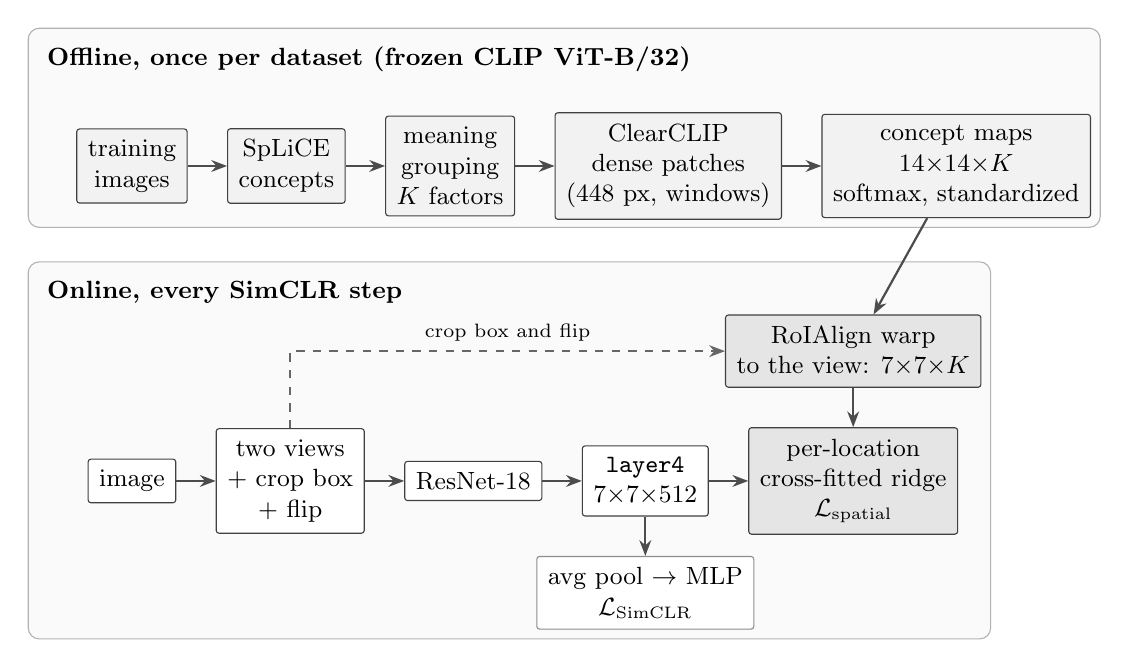
\begin{tikzpicture}[node distance=4mm and 5mm]
% offline teacher lane
\node[font=\small\bfseries,anchor=west] (offl) at (-0.3,1.35) {Offline, once per dataset (frozen CLIP ViT-B/32)};
\node[tbox] (t1) at (0.9,0) {training\\images};
\node[tbox,right=of t1] (t2) {SpLiCE\\concepts};
\node[tbox,right=of t2] (t3) {meaning\\grouping\\$K$ factors};
\node[tbox,right=of t3] (t4) {ClearCLIP\\dense patches\\(448 px, windows)};
\node[tbox,right=of t4] (t5) {concept maps\\$14{\times}14{\times}K$\\softmax, standardized};
\draw[arr] (t1)--(t2); \draw[arr] (t2)--(t3); \draw[arr] (t3)--(t4); \draw[arr] (t4)--(t5);
% online student lane
\node[font=\small\bfseries,anchor=west] (onl) at (-0.3,-1.6) {Online, every SimCLR step};
\node[sbox] (s1) at (0.9,-4.0) {image};
\node[sbox,right=of s1] (s2) {two views\\+ crop box\\+ flip};
\node[sbox,right=of s2] (s3) {ResNet-18};
\node[sbox,right=of s3] (s4) {\texttt{layer4}\\$7{\times}7{\times}512$};
\node[lbox,right=of s4] (s5) {per-location\\cross-fitted ridge\\$\mathcal L_{\text{spatial}}$};
\node[gbox,below=5mm of s4] (s6) {avg pool $\to$ MLP\\$\mathcal L_{\text{SimCLR}}$};
\node[lbox,above=5mm of s5] (warp) {RoIAlign warp\\to the view: $7{\times}7{\times}K$};
\draw[arr] (s1)--(s2); \draw[arr] (s2)--(s3); \draw[arr] (s3)--(s4); \draw[arr] (s4)--(s5); \draw[arr] (s4)--(s6);
\draw[arr] (t5)--(warp); \draw[arr] (warp)--(s5);
\draw[darr] (s2.north) |- node[above,font=\scriptsize,pos=0.75]{crop box and flip} (warp.west);
\begin{scope}[on background layer]
\node[fill=black!2,draw=black!30,rounded corners,fit=(offl)(t1)(t5)] {};
\node[fill=black!2,draw=black!30,rounded corners,fit=(onl)(s1)(s5)(s6)(warp)] {};
\end{scope}
\end{tikzpicture}
\caption{SCD. The teacher branch runs once (40 seconds on one GPU for MetaShift) and stores the maps. The
student branch adds one loss to unchanged SimCLR. At inference only the student backbone and the probe
remain; teacher, maps and heads are discarded.}
\label{fig:scd}
\end{figure}

\paragraph{Stages 1 and 2: concepts and concept factors.} SpLiCE codes $c_i$ (Section~\ref{sec:splice}) give the
vocabulary of the training set. The meaning grouping (Section~\ref{sec:grouping}) turns it into $K$ factors, each
with a text direction $d_F=\operatorname{norm}\big(\tfrac{1}{|F|}\sum_{k\in F}\operatorname{norm}(t_k)\big)$ and an
image-level activation $a_{iF}=\sum_{k\in F}c_{ik}$. Waterbirds has 242 factors, MetaShift 130 and Spur-CIFAR10 147.

\paragraph{Stage 3: dense concept maps.} Plain CLIP patch tokens of the last layer align poorly with text, because the
final attention mixes global information into every token \citep{zhou2022maskclip}. Following ClearCLIP
\citep{lan2024clearclip}, the last transformer block replaces its query--key attention by query--query attention and
drops its residual and feed-forward branches. With $X$ the normalized tokens entering this block, the patch
embeddings in the text space are
\begin{equation}
P=\operatorname{norm}\Big(\operatorname{LN}\big(\operatorname{softmax}(QQ^\top/\sqrt{d_h})\,V W_O\big)W_{\text{proj}}\Big),\qquad Q=XW_Q,\ V=XW_V,
\end{equation}
applied per attention head and normalized per patch. Images are read at 448 pixels through 224-pixel windows with a
stride of 112 pixels (Figure~\ref{fig:maps}); window scores are averaged where windows overlap and pooled to a
$14\times14$ grid. At every cell $u$ the map is a softmax over the factors,
\begin{equation}
M_{iF}(u)=\frac{\exp(\cos(p_i(u),d_F)/T)}{\sum_G\exp(\cos(p_i(u),d_G)/T)},\qquad \tilde M_{iF}=(M_{iF}-m_F)/s_F,
\end{equation}
with temperature $T=0.01$, so each cell distributes one unit of mass over the factors. Each factor's map is then
standardized over all images and cells ($m_F$, $s_F$) and stored in float16.

\begin{figure}[H]
\centering
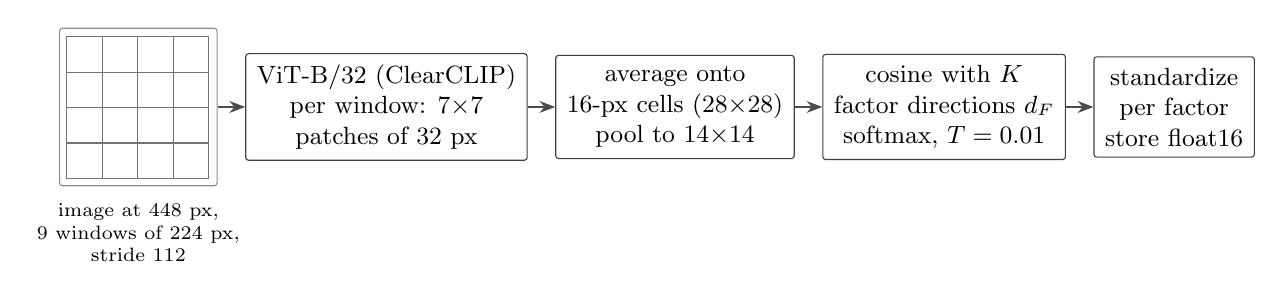
\begin{tikzpicture}[node distance=3.5mm]
\node[gbox,minimum width=20mm,minimum height=20mm] (img) {};
\foreach \i in {0,1,2} \foreach \j in {0,1,2} {
  \draw[black!55,thin] ($(img.south west)+(0.1+\i*0.45,0.1+\j*0.45)$) rectangle ++(0.9,0.9);
}
\node[below=1mm of img,font=\scriptsize,align=center] {image at 448 px,\\9 windows of 224 px,\\stride 112};
\node[box,right=of img] (vit) {ViT-B/32 (ClearCLIP)\\per window: $7{\times}7$\\patches of 32 px};
\node[box,right=of vit] (grid) {average onto\\16-px cells ($28{\times}28$)\\pool to $14{\times}14$};
\node[box,right=of grid] (cos) {cosine with $K$\\factor directions $d_F$\\softmax, $T=0.01$};
\node[box,right=of cos] (std) {standardize\\per factor\\store float16};
\draw[arr] (img)--(vit); \draw[arr] (vit)--(grid); \draw[arr] (grid)--(cos); \draw[arr] (cos)--(std);
\end{tikzpicture}
\caption{Map construction. Code: \texttt{cospro/pipeline/concept\_maps.py}; launcher:
\texttt{scripts/build\_concept\_maps.sbatch}.}
\label{fig:maps}
\end{figure}

\paragraph{Stage 4: warping the maps onto each view.} The standard two-view SimCLR objective remains unchanged. The
SSL transform records the crop box and flip of every view $x_i^{(v)}$. RoIAlign \citep{he2017maskrcnn} cuts the view's
box out of $\tilde M_i$ (a $2\times2$ sampling grid per output bin), resizes it to the student's feature map and flips
it with the view, giving targets $Y_i^{(v)}\in\mathbb R^{K\times h\times w}$ that describe exactly the pixels the view
shows. The feature map $H_i^{(v)}\in\mathbb{R}^{C\times h\times w}$ is the output of \texttt{layer4} before global
pooling ($7\times7\times512$ for 224-pixel views).

\paragraph{Stage 4: the per-location cross-fitted ridge.} Every location $u$ gives a unit-norm feature row
$r=\operatorname{norm}(H_i^{(v)}(u))\in\mathbb R^{512}$ and a target $y=Y_i^{(v)}(u)\in\mathbb R^K$. A trained linear
head on these rows could store a target per image, as the image-level heads did. We therefore split the images of a
batch into halves $A$ and $B$, with both views of an image in one half and fit a ridge regression on the locations of
$A$ in closed form,
\begin{equation}
W_A=\big(\bar R_A^\top\Omega_A\bar R_A+\rho I\big)^{-1}\bar R_A^\top\Omega_A(Y_A-\bar y_A),
\end{equation}
where $\bar R_A$ stacks the rows of $A$ centred by their weighted mean $\bar r_A$, $\Omega_A$ holds the per-view loss
weights and $\rho=1$ is an absolute ridge. The fit predicts every location of $B$, $\hat Y_B=(R_B-\bar r_A)W_A+\bar y_A$,
and the reverse fit predicts $A$. The loss is the held-out squared error,
\begin{equation}
\mathcal{L}_{\mathrm{spatial}}=\frac{1}{2}\sum_{(S,S')\in\{(A,B),(B,A)\}}
\frac{\sum_{v\in S'}\omega_v\,\frac{1}{hwK}\big\lVert\hat Y_v-Y_v\big\rVert_2^2}{\sum_{v\in S'}\omega_v}.
\end{equation}
Here the primal form is cheaper than the kernel form of Section~\ref{sec:xfit}: one $512\times512$ solve over
$64\cdot2\cdot49=6{,}272$ rows. The solve runs in float32 outside autocast. Gradients pass through the solve and the
prediction. A feature that identifies one image carries nothing to the other half; only concept directions shared
across images lower the loss.

A fixed fifth of the training images carries loss weight $\omega=0$: SimCLR still trains on them and they measure
whether the student carries concepts to images outside the concept loss. The complete objective is
\begin{equation}
\mathcal L=\mathcal L_{\text{SimCLR}}+\lambda(t)\,\mathcal L_{\text{spatial}},\qquad \lambda(t)=0 \text{ up to epoch 10, linear to } \lambda_{\max}=5 \text{ at epoch 20.}
\end{equation}

\paragraph{One training step.}
\begin{enumerate}[leftmargin=*]
\item Draw 128 images, two augmented views each; record each view's crop box and flip.
\item Run the student; keep the pooled vector for SimCLR and the $7\times7\times512$ \texttt{layer4} map from the hook.
\item Warp each image's stored $14\times14\times K$ map to each view's box and flip: $7\times7\times K$ targets.
\item Split the images into halves; fit the ridge on all locations of one half, predict the other, both directions.
\item Add $\lambda(t)$ times the held-out error to the SimCLR loss and back-propagate through the solve.
\end{enumerate}

\subsection{Design choices and their justification}
\begin{itemize}[leftmargin=*]
\item \textbf{ClearCLIP as the dense teacher.} Training-free dense CLIP methods give patch--text alignment without
any segmentation labels \citep{zhou2022maskclip,wang2024sclip,lan2024clearclip}; ClearCLIP reports the highest
open-vocabulary segmentation scores of the three and keeps the restriction (no labels).
\item \textbf{448 pixels through 224-pixel windows with stride 112.} ViT-B/32 sees a 224-pixel input as only
$7\times7$ patches of 32 pixels, too coarse to separate a cat from its cushion. Sliding-window inference with
224-pixel windows and stride 112 on an enlarged image follows the evaluation of SCLIP and ClearCLIP
\citep{wang2024sclip,lan2024clearclip}; it gives an effective 16-pixel grid while each window stays at the resolution
CLIP was trained on.
\item \textbf{$14\times14$, twice the student's $7\times7$.} A SimCLR crop covers 20\% to 100\% of the image; a 20\%
crop still spans about $6\times6$ map cells, so RoIAlign has real content to resample into the $7\times7$ target.
\item \textbf{Softmax with $T=0.01$.} CLIP's learned logit scale is 100 \citep{radford2021clip}, which is a
temperature of 0.01; its zero-shot classifier applies this scale to the same cosines. Cosines of a patch with
different text directions differ by a few hundredths and $T=0.01$ turns them into a peaked distribution, so each cell
mostly picks a winner.
\item \textbf{Standardized per factor.} Every factor then has unit variance, so frequent factors (blanket, lawn) do
not dominate the squared error.
\item \textbf{RoIAlign for the warp.} RoIAlign samples the map at exact fractional coordinates with bilinear
interpolation \citep{he2017maskrcnn}; it keeps the map aligned with the view's pixels for any crop box.
\item \textbf{Cross-fit in place of a trained head}: the lesson of the image-level line, where a trained head stored
per-image targets on small datasets.
\item \textbf{$\lambda_{\max}=5$}: from the weight grid 1, 3, 5 and 10 of the image-level loss; spatial weight 10 adds
nothing (Waterbirds 53.5, MetaShift 48.3, two seeds).
\item \textbf{Start at epoch 10 with a 10-epoch warm-up}: SimCLR forms features before the concept loss acts;
inherited from F2, where starting at epoch 0 changed nothing.
\item \textbf{20\% hold-out}: introduced as a diagnostic. The arm with the hold-out scored higher than the arm
without it (Waterbirds 52.8 vs.\ 49.5, MetaShift 51.1 vs.\ 46.7, six seeds) and became the main arm. The difference
lies within the seed spread and has no explanation yet.
\item \textbf{Batch 128}: 6,272 rows per half against 512 dimensions keep the fit well posed.
\end{itemize}

\subsection{Experimental protocol}
We evaluate on Waterbirds, MetaShift cats and dogs and Spur-CIFAR10. Each dataset gets its own concept factors and
maps from its training images. We pretrain a randomly initialized ResNet-18 for 500 epochs with batch size 128, the
same augmentations and optimization schedule for every method and SimCLR temperature 0.05. The concept loss uses ridge
$\rho=1$, weight 5 and the 20\% hold-out. We report six student seeds on Waterbirds and MetaShift and two on
Spur-CIFAR10. Frozen student features are evaluated every 25 epochs with the same logistic probe, fitted on the
group-balanced subset of the training split. Each value is the mean of the last four probes (epochs 425 to 500). We
report mean and sample standard deviation across student seeds and paired differences per seed
\citep{bouthillier2021variance}.

\subsection{Results}
\begin{table}[H]
\centering
\caption{SCD against SimCLR and the shuffled-map control. Waterbirds and MetaShift: seeds 1--6; Spur-CIFAR10:
seeds 1--2. Validation, mean of the last four probes.}
\label{tab:scd}
\small
\begin{tabular}{lcccccc}
\toprule
 & \multicolumn{2}{c}{Waterbirds} & \multicolumn{2}{c}{MetaShift} & \multicolumn{2}{c}{Spur-CIFAR10} \\
Method & Avg. & WGA & Avg. & WGA & Avg. & WGA \\
\midrule
SimCLR & 52.4 & \pmsd{46.7}{1.9} & 55.2 & \pmsd{44.3}{7.3} & 59.6 & \pmsd{15.6}{1.0} \\
Shuffled maps & 52.8 & \pmsd{47.5}{2.5} & 56.1 & \pmsd{45.1}{2.9} & 55.9 & \pmsd{17.3}{2.0} \\
\textbf{SCD} & \textbf{60.3} & \textbf{\pmsd{52.8}{4.7}} & \textbf{61.2} & \textbf{\pmsd{51.1}{5.4}} & \textbf{69.3} & \textbf{\pmsd{38.1}{0.5}} \\
\bottomrule
\end{tabular}
\end{table}

SCD beats SimCLR by 6.1 (Waterbirds), 6.8 (MetaShift) and 22.5 (Spur-CIFAR10) points of WGA and by 7.9, 6.0 and 9.8
points of average accuracy. It is ahead on five of six paired seeds on Waterbirds and MetaShift and on both
Spur-CIFAR10 seeds (Table~\ref{tab:paired}). The shuffled control stays within one point of SimCLR on Waterbirds and
MetaShift and 1.6 points on Spur-CIFAR10, so the gain comes from the content of each image's own maps. The gain
extends to the minority groups: on MetaShift cats outdoors rise from 47.0 to 51.2 and dogs indoors from 52.8 to 57.2;
on Waterbirds landbirds on water rise from 53.6 to 65.1 (Appendix~\ref{app:seeds}).

\begin{table}[H]
\centering
\caption{Paired SCD differences in percentage points per seed, mean of the last four probes.}
\label{tab:paired}
\small
\begin{tabular}{rrrrrrrrr}
\toprule
& \multicolumn{4}{c}{Waterbirds} & \multicolumn{4}{c}{MetaShift} \\
& \multicolumn{2}{c}{vs. SimCLR} & \multicolumn{2}{c}{vs. shuffled maps} & \multicolumn{2}{c}{vs. SimCLR} & \multicolumn{2}{c}{vs. shuffled maps} \\
Seed & $\Delta$Avg. & $\Delta$WGA & $\Delta$Avg. & $\Delta$WGA & $\Delta$Avg. & $\Delta$WGA & $\Delta$Avg. & $\Delta$WGA \\
\midrule
1 & +9.30 & +12.29 & +3.50 & +7.07 & +9.72 & +9.72 & +7.99 & +17.36 \\
2 & +11.45 & +7.34 & +10.15 & +3.59 & +3.56 & +5.90 & +4.60 & +8.68 \\
3 & +6.80 & +3.32 & +7.09 & +5.84 & +13.54 & +22.57 & +4.69 & +4.86 \\
4 & +4.05 & +5.97 & +9.47 & +8.69 & +2.86 & $-$5.21 & +9.11 & +0.00 \\
5 & +11.41 & +10.47 & +10.36 & +10.57 & +6.51 & +4.17 & +1.48 & +2.08 \\
6 & +4.30 & $-$2.78 & +4.61 & $-$4.18 & $-$0.26 & +3.47 & +2.60 & +3.13 \\
\midrule
Mean & +7.88 & +6.10 & +7.53 & +5.26 & +5.99 & +6.77 & +5.08 & +6.02 \\
\bottomrule
\end{tabular}
\end{table}

\begin{figure}[H]
\centering
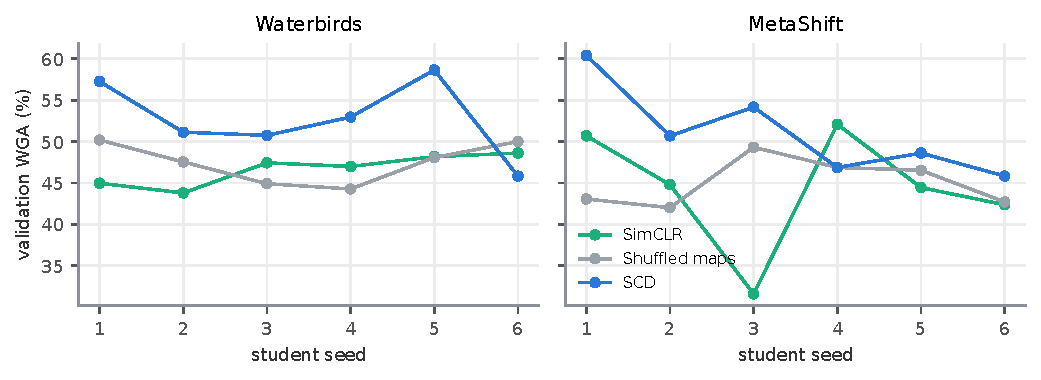
\includegraphics[width=0.92\linewidth]{figures/paired_seeds.pdf}
\caption{Per-seed WGA. MetaShift seeds spread by more than 20 points for SimCLR (31.6 to 52.1), which is why
we report six seeds and paired differences. Seed 6 is hard for every method on Waterbirds.}
\label{fig:seeds}
\end{figure}

\begin{figure}[H]
\centering
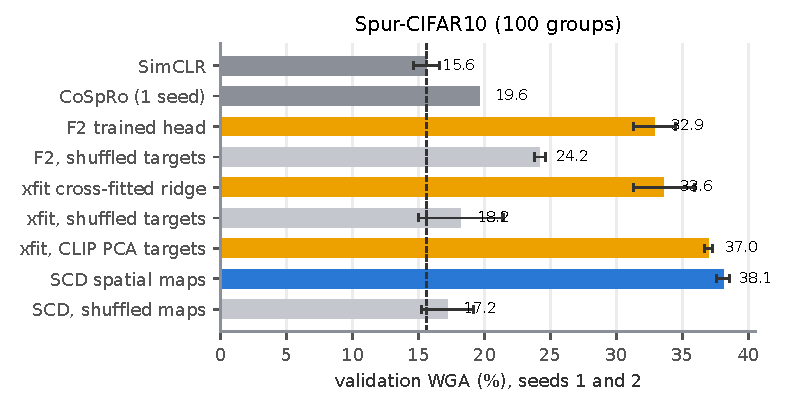
\includegraphics[width=0.75\linewidth]{figures/spur_cifar10.pdf}
\caption{Spur-CIFAR10, where the spurious feature is a thin coloured line. Every real-target method roughly
doubles WGA and every shuffled control stays near SimCLR. SCD gives the best result of the branch.}
\label{fig:cifar}
\end{figure}

The advantage holds across training (Figure~\ref{fig:curves}). On MetaShift the smoothed mean WGA of SCD leads all
other methods at every probe from epoch 100 onward; from epoch 200 its margin over the closest method ranges from 3.4
to 8.0 points. On Waterbirds SCD leads SimCLR and the shuffled control from epoch 100 onward and the
principal-component maps follow the same path. Average accuracy separates earlier: SCD leads all methods on both
datasets from epoch 125 onward.

\begin{figure}[H]
\centering
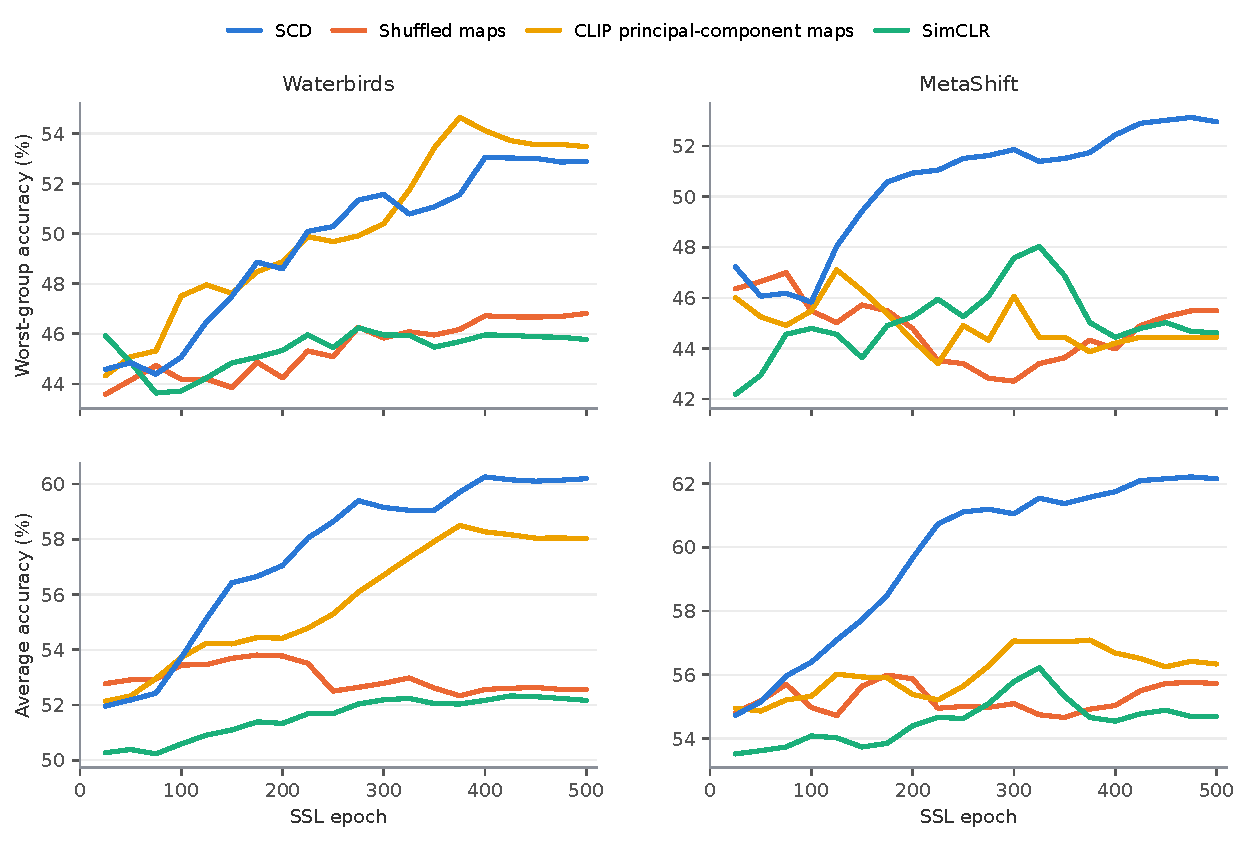
\includegraphics[width=0.95\linewidth]{figures/spatial_training_curves.pdf}
\caption{Validation accuracy during SSL training (seeds 1--4, 3-point smoothing). Top: WGA; bottom: average accuracy.}
\label{fig:curves}
\end{figure}

\subsection{Controls: concepts, CLIP or location?}
Three controls separate the ingredients of SCD. The principal-component control replaces the concept maps by as many
principal components of the dense ClearCLIP patch embeddings as there are factors, computed over the same cells and
trained with the same loss: it keeps the dense CLIP information of the teacher and removes the concept names. The
image-level control regresses each image's SpLiCE factor activations from the pooled features with the same
cross-fitted ridge and weight: it keeps the concepts and removes their locations. A concept ablation removes groups
of factors.

\begin{table}[H]
\centering
\caption{Controls of SCD, seeds 1--4 (image-level row on MetaShift: seeds 1--2).}
\label{tab:controls}
\small
\begin{tabular}{lcccc}
\toprule
 & \multicolumn{2}{c}{Waterbirds} & \multicolumn{2}{c}{MetaShift} \\
Method & Avg. & WGA & Avg. & WGA \\
\midrule
SimCLR & 52.3 & \pmsd{45.8}{1.7} & 54.8 & \pmsd{44.8}{9.4} \\
Shuffled maps & 52.6 & \pmsd{46.7}{2.7} & 55.6 & \pmsd{45.3}{3.4} \\
CLIP principal-component maps & 58.1 & \pmsd{53.6}{1.9} & 56.3 & \pmsd{44.4}{7.4} \\
Image-level factor regression & 58.0 & \pmsd{50.4}{9.0} & 61.7 & \pmsd{47.2}{3.9} \\
SCD & 60.2 & \pmsd{53.0}{3.0} & 62.2 & \pmsd{53.0}{5.8} \\
\bottomrule
\end{tabular}
\end{table}
\begin{itemize}[leftmargin=*]
\item \textbf{Principal-component maps.} On MetaShift SCD wins on all four seeds ($+16.0$, $+1.4$, $+4.2$, $+12.9$); the PCA
maps stay at the SimCLR level. On Waterbirds the two tie: birds against land and water are among the strongest
directions of CLIP's patch space, so the leading components carry them; cats against dogs and couches against lawns
are weaker directions that only the named concepts single out.
\item \textbf{Image-level regression.} SCD is ahead by 2.7 WGA on Waterbirds, 8.3 on the two paired MetaShift seeds
and 8.7 on Spur-CIFAR10 (29.4 against 38.1).
\item \textbf{Concept ablation} on MetaShift (seeds 1--4), an analysis with word lists we chose, outside the method:
without the 21 animal factors \pmsd{46.6}{5.8}, without the 20 scene factors \pmsd{47.9}{2.8}, all factors
\pmsd{53.0}{5.8}. Both ablations lose most of the gain: it needs the full concept set.
\end{itemize}

\subsection{What the student learns}
\label{sec:audit}
\begin{figure}[H]
\centering
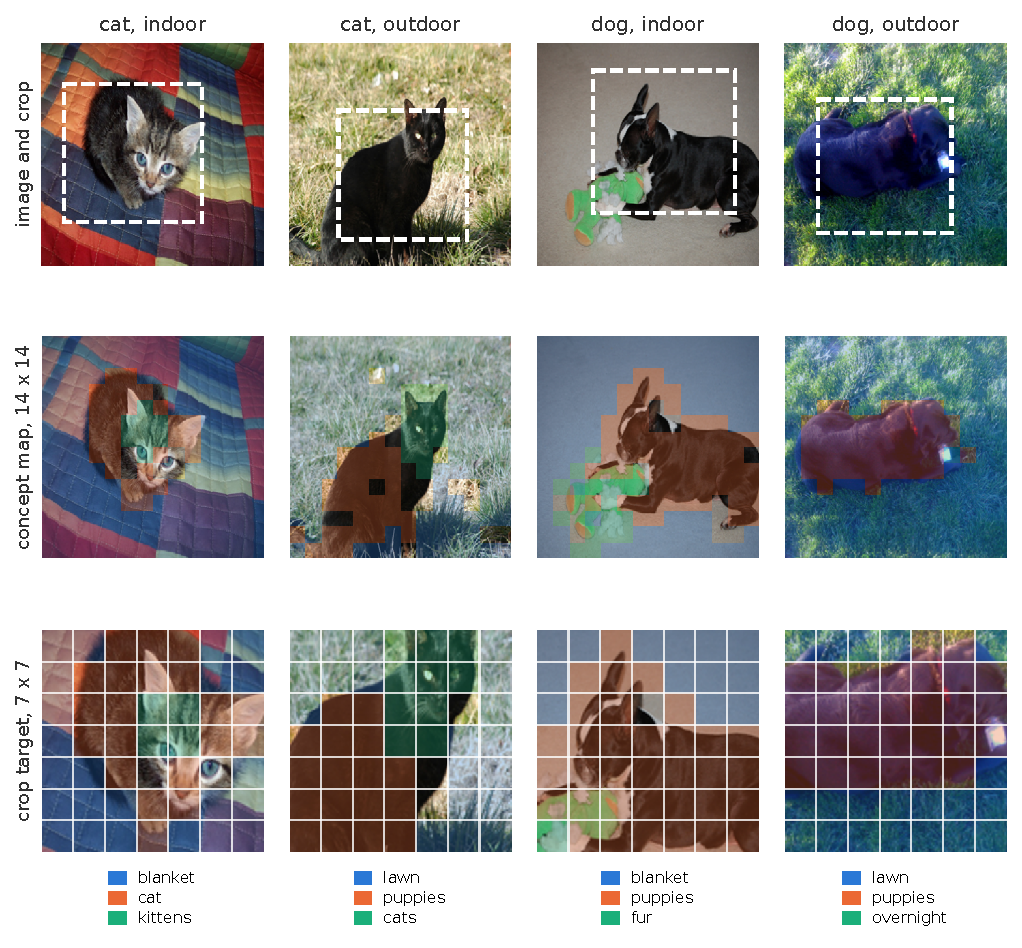
\includegraphics[width=0.82\linewidth]{figures/spatial_map_examples.pdf}
\caption{MetaShift concept maps. Top: image and one SimCLR crop (dashed). Middle: the winning factor of each
of the $14\times14$ cells (the three most frequent factors coloured). Bottom: the crop's $7\times7$ targets after
warping. The animal factors cover the animal, the scene factors its surroundings. The teacher is imperfect:
in the cat-outdoor image part of the black cat is labelled ``puppies''.}
\label{fig:mapexamples}
\end{figure}

\textbf{What the maps contain.} The MetaShift factors include scene concepts such as couch, lawn, beds, windows and
bench next to the animal concepts; blankets, lawn, cats and fields win the most map cells (7.4\%, 6.6\%, 5.8\% and
5.6\%). On Waterbirds bamboo, forest and tree stand win 37\% of the cells and the factor \emph{water bird} 6.2\%.

\textbf{The student generalizes.} On the held-out fifth the student's pooled features explain 0.22 (MetaShift) and
0.26 (Waterbirds) of the image-level factor responses, against 0.13 and 0.17 with shuffled maps; scores on images
inside the loss agree (0.23 and 0.26). The memorization of the image-level line is gone
(Figure~\ref{fig:memorization}).

\textbf{The student keeps the co-occurrence.} With labels used only for this audit, the student's \emph{cat} factor
scores 0.47 on unseen cats indoors and 0.07 on unseen cats outdoors; CLIP scores 0.92 and 0.88
(Figure~\ref{fig:decoupling}). The factor residuals score 0.00 in the student against 0.15 to 0.17 for CLIP. A
background probe on the frozen features reaches 90.5\% WGA for SCD against 89.5\% for SimCLR: SCD keeps the
background as readable as before. Correlated generative factors in the training data persist in learned
representations \citep{trauble2021correlated} and each $7\times7$ location sees most of the view
(Section~\ref{sec:resnet}); the cheapest predictor of ``cat here'' therefore combines local evidence with the scene,
which agrees with the cat on 88\% of the training images.

\begin{figure}[H]
\centering
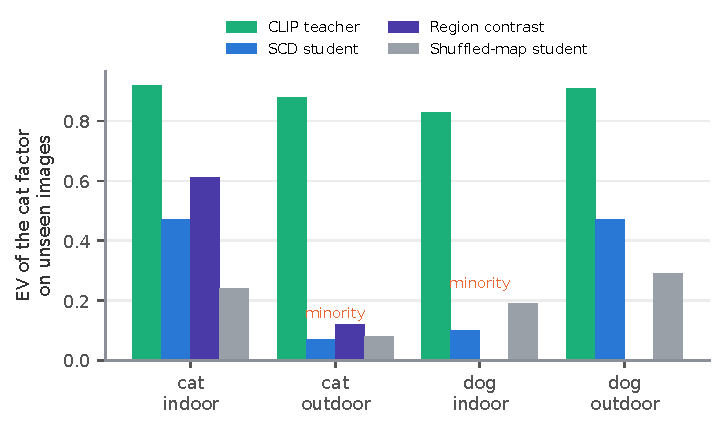
\includegraphics[width=0.62\linewidth]{figures/decoupling.pdf}
\caption{How well the \emph{cat} factor is predicted on unseen MetaShift images, per group. CLIP sees cats
everywhere; every student sees cats where cat and scene agree (cat indoors) and fails on the minority groups.}
\label{fig:decoupling}
\end{figure}

\begin{figure}[H]
\centering
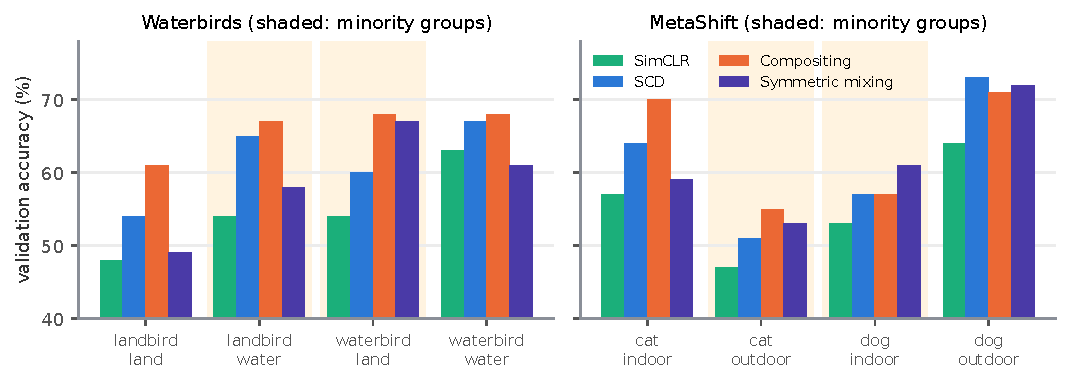
\includegraphics[width=0.95\linewidth]{figures/group_accuracies.pdf}
\caption{Accuracy per group (six seeds for SimCLR and SCD; compositing six seeds on Waterbirds, four on
MetaShift; mixing four). SCD raises every group, the minority groups included; compositing flattens the
Waterbirds groups at 61 to 68.}
\label{fig:groups}
\end{figure}

\subsection{Limitations of SCD}
All results are validation results with the probe evaluated on the same split; the locked test runs are prepared. The
weight $\lambda_{\max}=5$ and the hold-out were chosen on the validation splits of MetaShift and Waterbirds with seeds
1--4; seeds 5 and 6 ran with the settings fixed. MetaShift's seed spread (5.4 WGA points) is as large as the gain over
its controls on single seeds. On Waterbirds dense CLIP components match the concept maps, so the concept names add
value only where the relevant contrast is a weak direction of CLIP. The method depends on CLIP's external
pretraining, its vocabulary and its 32-pixel patches: Spur-CIFAR10 images are upsampled from 32 to 448 pixels for the
maps and CelebA has no concept maps yet.

\subsection{Conclusion on SCD}
SCD uses dense maps of SpLiCE concepts to supervise every location of a SimCLR student through a regression
cross-fitted between halves of the batch, with no labels and no concept type during pretraining. On Waterbirds,
MetaShift and Spur-CIFAR10 its mean validation worst-group and average accuracies exceed those of SimCLR and of the
same loss on shuffled maps. On MetaShift the named concepts beat dense CLIP components of the same width; on
Waterbirds the two tie. SCD raises WGA because the balanced probe gains a usable core feature that SimCLR from scratch
lacks, while the student's concepts still follow the training co-occurrence. SCD is the prior-free method of the
thesis.

%=====================================================================
\section{Separating object and context}
\label{sec:objectcontext}
%=====================================================================
Every loss so far is an expectation over the natural training images, where cats sit indoors. The four extensions of
this section either change that distribution or demand that a concept keeps its identity in other surroundings. All
four run on top of SCD (weight 5, 20\% hold-out). The theoretical motivation is the content--style result of
\citet{vonkugelgen2021content}: contrastive learning isolates the content that its augmentations keep fixed, provided
the augmentations change the style independently of it. Natural crops never move a cat outdoors, so the scene stays
part of the ``content''.

\subsection{Region contrast (DetCon-style)}
\summary The feature map is pooled inside each view's dominant concept regions and the pooled regions are contrasted
across the batch, so that a cat region on a lawn must resemble a cat region on a couch. The concept scores on unseen
images rise on every seed, yet WGA moves within noise ($+2.3$ on Waterbirds, $-3.0$ on MetaShift against SCD on the
same seeds) and the gain goes to the majority groups. Region pooling inherits the receptive-field problem of
Section~\ref{sec:resnet}: a region feature still sees the scene and on Waterbirds a shuffled region arm gains as much
as the real one.

\textbf{Method.} Following DetCon \citep{henaff2021detcon}, each view's feature map is pooled inside its two dominant
concept regions (warped map probability as weight, mean probability at least 0.1), projected with a small head and
contrasted across the batch: regions of the same concept in other images are positives, weighted towards pairs whose
images' concept mixes differ. About 335 regions form per MetaShift batch, 94\% of them with positives.

\textbf{Result.} Waterbirds \pmsd{55.3}{3.1} (SCD 53.0 on the same seeds), MetaShift \pmsd{50.0}{6.5} (below SCD on three
of four seeds). The concept scores on unseen images rise on every seed (MetaShift 0.22 $\to$ 0.29) and the cat factor
on cats outdoors from 0.05 to 0.12. On Waterbirds the shuffled region arm gains as much over shuffled SCD as the real
one over SCD: part of the gain is region pooling itself.

\subsection{Concept compositing (with the object prior)}
\summary The object region of one image is cut out and pasted onto the context of another image, whose own objects are
painted over; the composite replaces the second SimCLR view. With a random donor, object and context become
independent in the composites. It works best of all variants: Waterbirds 59.1 WGA, ahead of SCD on all six seeds, and
the steadiest MetaShift result (52.3, sd 1.9). It needs a text prior that types each concept as an object or a scene,
which the restriction excludes; compositing therefore measures what a correct prior adds.

\textbf{Method.} For 30\% of the qualifying images, the \emph{object} region of the second view is cut out and pasted
onto another image's view whose own objects are painted over by normalized convolution from their surroundings
\citep{knutsson1993normalized}. Cut-and-paste synthesis is an established augmentation for detection and segmentation
\citep{dwibedi2017cutpaste,ghiasi2021copypaste}; DiLo and object-aware contrastive learning paste salient objects onto
other backgrounds during SSL \citep{zhao2021dilo,mo2021objectaware}. The concept targets are composited with the same
mask. With a random donor, the composites sample the interventional distribution in which the context carries no
information about the object \citep{pearl2009causality}; augmentations that simulate such interventions yield
invariance to the intervened factor \citep{ilse2021interventions,mitrovic2021relic}, which is the content--style
condition of \citet{vonkugelgen2021content}.

\textbf{Which concepts are ``objects''} is decided by text alone (\texttt{cospro/pipeline/concept\_type.py}): CLIP
text similarity to scene prompts minus similarity to object prompts; factors below the median count as objects. No
label enters, but the step \emph{types} concepts. On MetaShift the 65 object factors hold every animal and breed (and
also verbs and people); lawn, couch, bed, desk, window, beach and snow are context.

\begin{figure}[H]
\centering
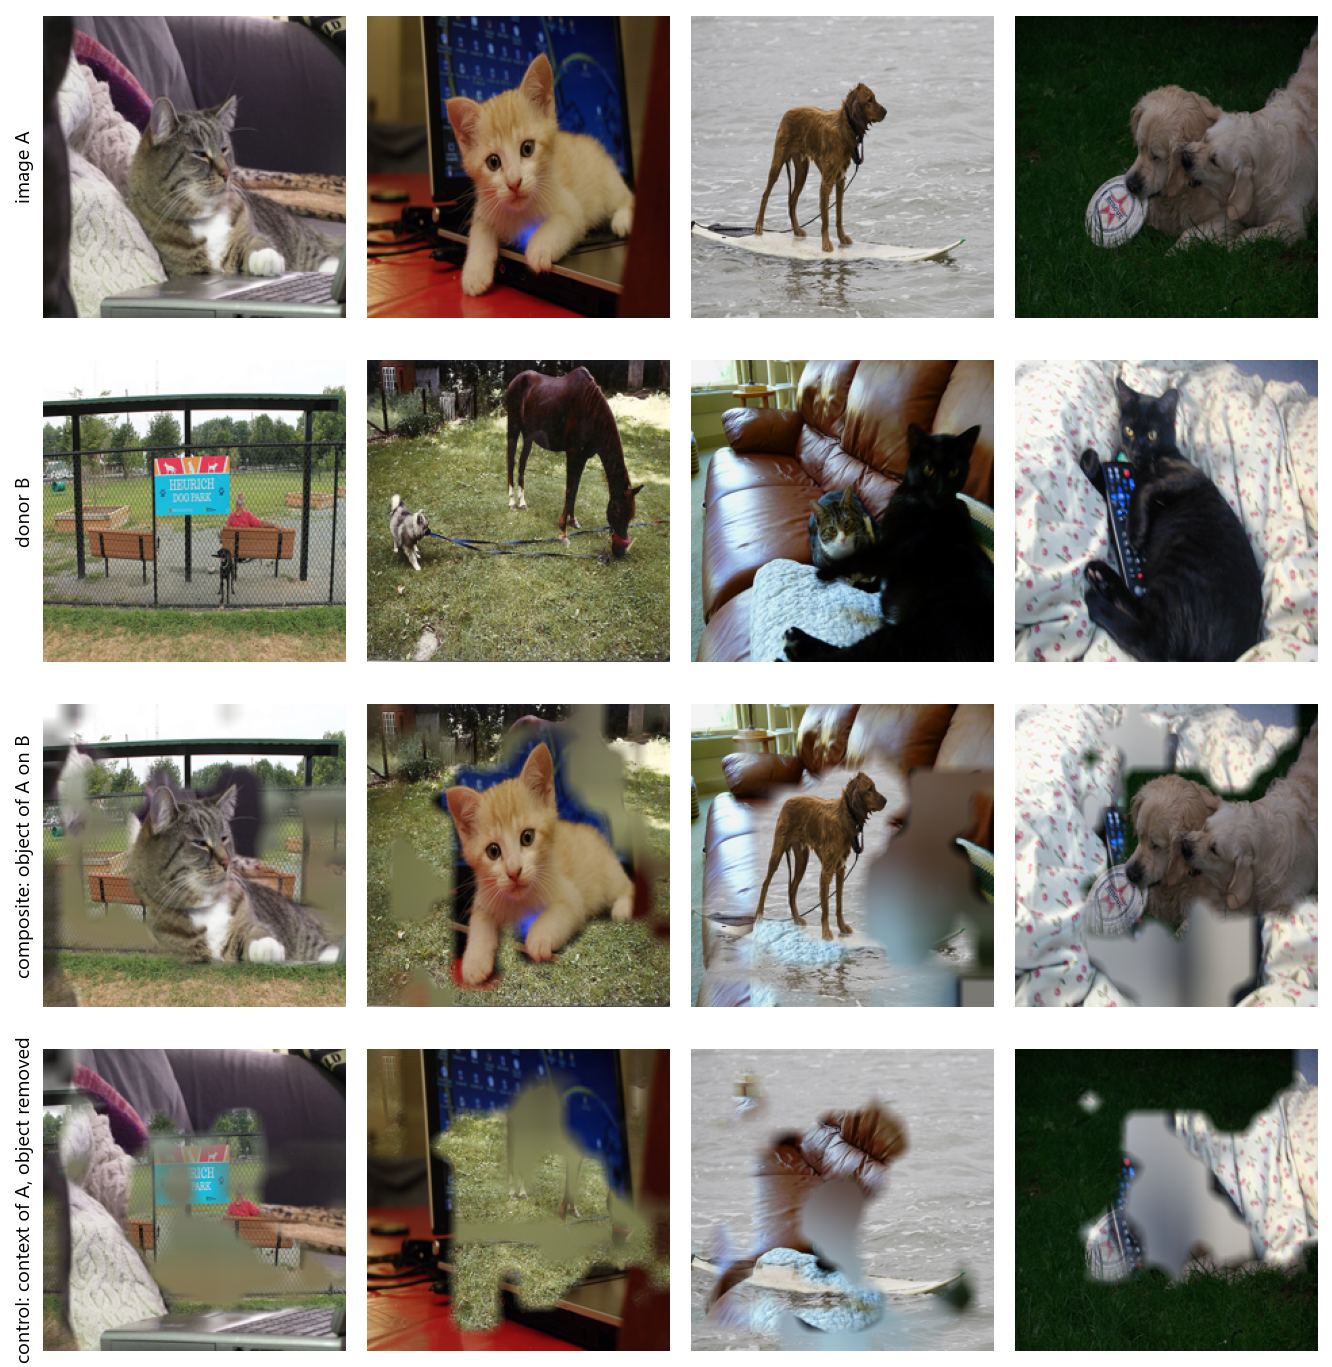
\includegraphics[width=0.72\linewidth]{figures/composites_metashift.png}
\caption{Real MetaShift composites. Row 3: the object of image A on donor B (the training input). Row 4: the
``context kept'' control, which pastes A's surroundings instead. Seams are half a map cell wide.}
\label{fig:composites}
\end{figure}

\begin{figure}[H]
\centering
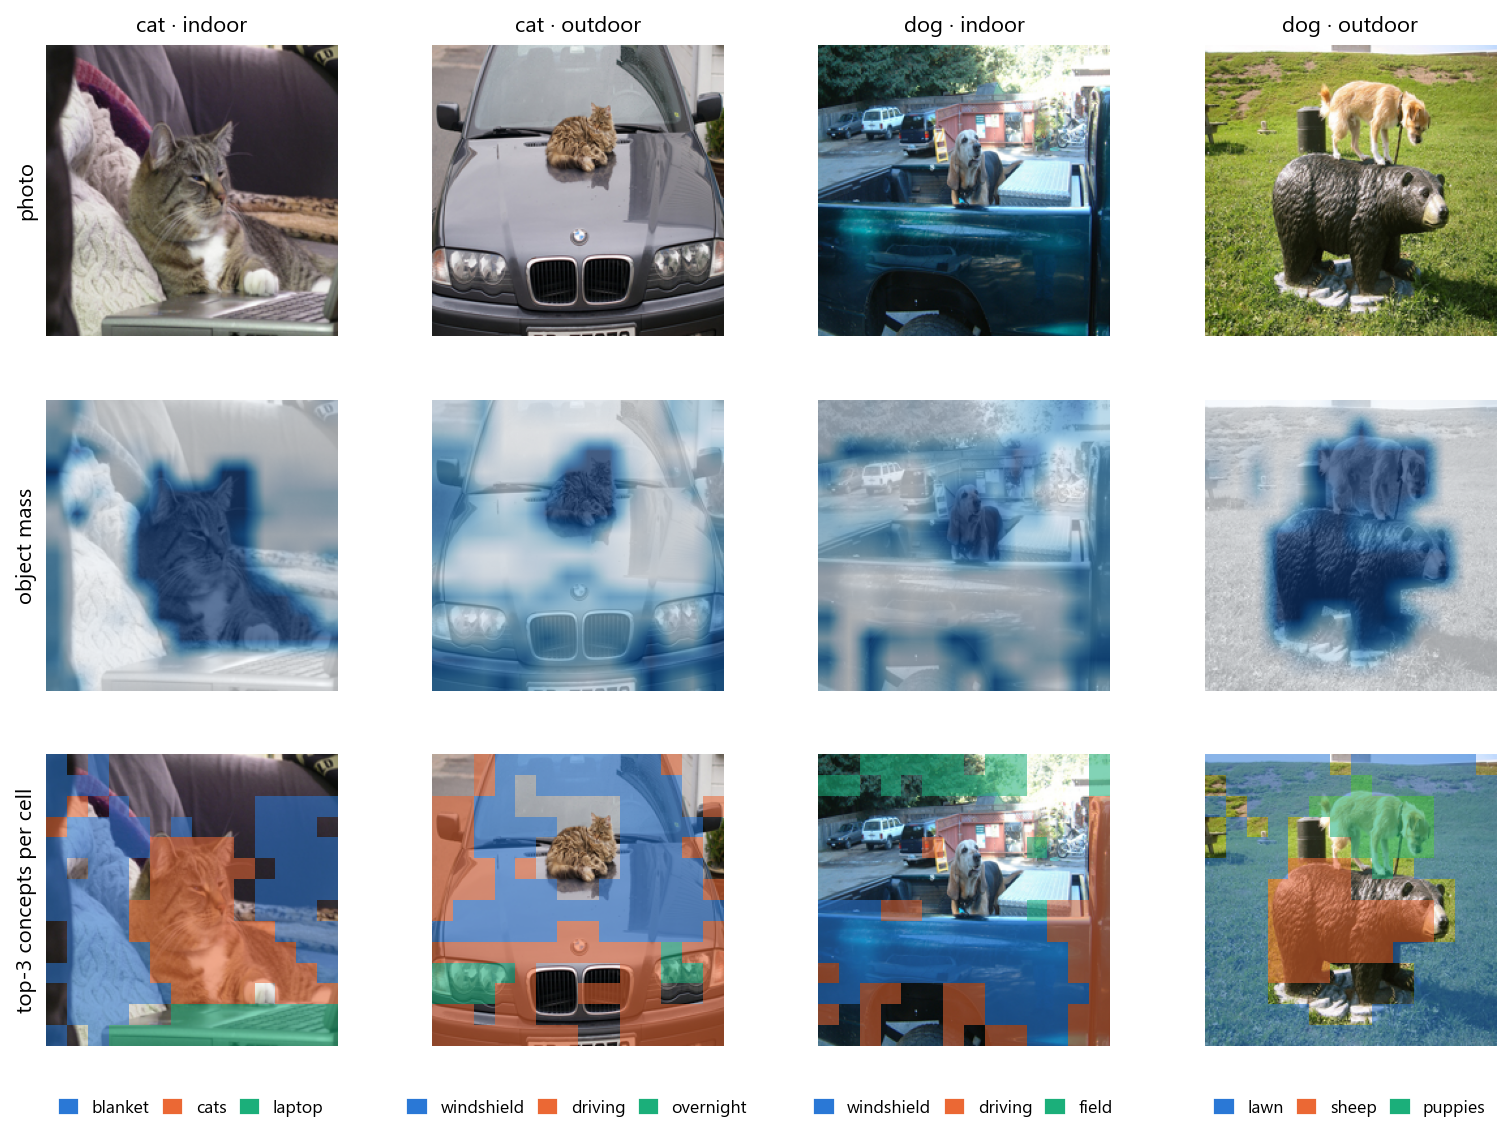
\includegraphics[width=0.78\linewidth]{figures/concept_maps_metashift.png}
\caption{The object mass that compositing cuts (row 2) and the three leading concepts per cell (row 3) on
one MetaShift image per group. The teacher often names the context well (windshield, driving, lawn) and
the animal in broad strokes.}
\end{figure}

\begin{table}[H]
\centering
\caption{Compositing and its controls (validation WGA / Avg.). Waterbirds seeds 1--6 for compositing and the
silhouette control, 1--4 otherwise; MetaShift seeds 1--4.}
\small
\begin{tabular}{lcc}
\toprule
Arm & Waterbirds & MetaShift \\
\midrule
SCD & 52.8 / 60.3 & 51.1 / 61.2 \\
\textbf{Compositing, object regions} & \textbf{\pmsd{59.1}{7.1}} / 64.7 & \pmsd{52.3}{1.9} / 63.3 \\
\quad control: another image's object silhouette & \pmsd{54.2}{6.1} / 62.5 & \pmsd{50.6}{3.7} / 60.0 \\
\quad control: context region pasted instead & \pmsd{52.7}{2.1} / 60.0 & \pmsd{49.3}{1.9} / 60.1 \\
\quad control: shuffled maps & \pmsd{52.9}{1.0} / 57.2 & \pmsd{48.4}{3.1} / 56.6 \\
\bottomrule
\end{tabular}
\end{table}

\textbf{Result.} On Waterbirds compositing beats SCD on all six seeds (6.3 WGA on average), the context and shuffled
controls on all four paired seeds and the silhouette control on four of six; its groups flatten to 61--68. On
MetaShift it gives the steadiest WGA of the branch (sd 1.9). The arms order as the concept hypothesis predicts: object
regions $>$ random silhouettes $>$ context regions. The gain rests on the object prior (target = object, spurious
attribute = surroundings), which the restriction excludes and which CelebA breaks. Background augmentations report the
same kind of gain under the same prior \citep{ryali2021background}.

\subsection{Symmetric concept mixing (no prior)}
\summary The prior-free version of compositing: every concept region of an image is kept or replaced at random, so no
concept is typed. It falls below SCD on Waterbirds (49.2), ties it on MetaShift (51.0) and ties its own control with
random rectangles on both datasets. Without the object type the method reduces to CutMix-like mixing: half of the
mixes keep the scene and replace the cat, which teaches the scene as much as the cat.

\textbf{Method.} Each concept region of view A is kept with probability one half (kept area 25--75\%) and the rest
filled from a random donor B: $x=M\odot A+(1-M)\odot B$, as in CutMix \citep{yun2019cutmix} with concept-shaped masks.
The mixed view is a third encoder pass. Its feature map pooled inside $M$ is a positive of A and pooled outside a
positive of B, as in RegionCL \citep{xu2022regioncl}; its global embedding is a soft positive of A and B in proportion
to their areas, as in Un-Mix \citep{shen2022unmix}. Under mixing the twelve strongest animal-by-scene correlations on
MetaShift fall from mean $|\phi|=0.33$ to 0.19 (object pasting: 0.17).

\textbf{Result.} Waterbirds \pmsd{49.2}{2.5} (below SCD on all four seeds), MetaShift \pmsd{51.0}{8.5}; it ties its
rectangle control on both datasets (49.0 and 51.8), so concept boundaries make no difference. The mixing weakens the
majority group landbird-on-land (49 vs.\ 55).

\subsection{Per-group projection heads (LooC-style, no prior)}
\summary Symmetric mixing asks one embedding to stay the same whatever part was replaced, sometimes the scene and
sometimes the cat and these demands may cancel. Separate projection heads per concept group remove the conflict.
The heads train well (the highest unseen concept scores of all arms), but the effect changes sign between datasets:
Waterbirds 52.4 (ties SCD), MetaShift 46.9 (below SCD by 6.2). The class groups are kept in only 21\% of the mixes,
and drawing them more often would require knowing the class, which is the prior again. This ended the prior-free
mixing line.

\textbf{Method.} LooC gives each invariance its own embedding space \citep{xiao2021looc}. Factors are clustered into 12
groups by the pixels they share in the maps (spectral clustering of map co-activation, \citealp{ng2001spectral}; no
label or prompt). For half of the images one group is kept on a donor; the mix is a positive of its image only in that
group's own projection head.

\textbf{Result.} Waterbirds \pmsd{52.4}{2.9} (ties SCD, beats the single-head control by 9.5); MetaShift \pmsd{46.9}{3.3}
(below the single head by 5.2, below SCD by 6.2 and below its shuffled control). Concept scores on unseen images
(0.28 and 0.32) do not predict WGA.

%=====================================================================
\section{Comparison of all architectures}
\label{sec:scoreboard}
%=====================================================================
\begin{table}[H]
\centering
\caption{All architectures with their idea, outcome and the lesson they taught. WGA on Waterbirds / MetaShift
(validation).}
\small
\begin{tabularx}{\linewidth}{>{\raggedright\arraybackslash}p{2.6cm} >{\raggedright\arraybackslash}X c >{\raggedright\arraybackslash}X}
\toprule
Architecture & Idea & WGA (WB / MS) & Lesson \\
\midrule
F2 trained head & regress factor values from the pooled feature & 41.6 / 46.6 & per-image targets are memorized on small datasets \\
F3 concept blocks & SupCon per factor, cross-context positives & -- / 43.8 & shuffled concept sets fit as well \\
xfit & ridge fitted on one half, tested on the other & 51.5 / 47.6 & removes head memorization; backbone still memorizes; CLIP PCA as good \\
\textbf{SCD} & per-location cross-fit on dense concept maps & \textbf{52.8 / 51.1} & location helps; generalizes; keeps the co-occurrence \\
Region contrast & DetCon over concept regions & 55.3 / 50.0 & raises concept scores, minority groups stay \\
\textbf{Compositing} & paste object on another scene & \textbf{59.1 / 52.3} & works, needs object-vs-scene prior \\
Symmetric mixing & keep random concept regions, soft positives & 49.2 / 51.0 & equals CutMix with rectangles \\
Per-group heads & one embedding space per concept group & 52.4 / 46.9 & sign flips; drawing the class needs the prior \\
\bottomrule
\end{tabularx}
\end{table}

%=====================================================================
\section{Interpretation}
%=====================================================================
\begin{enumerate}[leftmargin=*]
\item \textbf{Concepts help a from-scratch SSL student when they are delivered where they are.} Image-level
distillation is limited by memorization and by co-occurrence; spatial distillation generalizes and lifts every group.
\item \textbf{Every claim stands on a matched control.} Shuffled targets test content, PCA maps test named concepts
against generic CLIP information, image-level regression tests location and ablations test which concepts matter.
\item \textbf{The core feature becomes stronger and stays fused with its context.} DFR needs separate directions; SCD
supplies a stronger core direction that still carries the scene. Loosening the fusion worked only with an object
prior.
\item \textbf{The decision for the thesis.} The prior-free method is SCD. Compositing reports what a correct assumption
about the spurious attribute adds, stated openly, as the background-augmentation literature does
\citep{ryali2021background}.
\end{enumerate}

%=====================================================================
\section{Limitations and next steps}
%=====================================================================
\begin{itemize}[leftmargin=*]
\item \textbf{Validation only.} Model selection on the evaluation split inflates results
\citep{gulrajani2021lost}. \texttt{FINAL\_TEST=1 bash scripts/submit\_factor\_study.sh <dataset>} runs the same arms once
on the locked test split (Waterbirds test: 642 images per minority group against 133 in validation).
\item \textbf{Noise.} MetaShift's seed spread (5.4 WGA) is as large as the gain on single seeds.
\item \textbf{The hold-out effect} (higher WGA with 20\% of images out of the concept loss) has no explanation.
\item \textbf{LateTVG matched comparison}: one seed under our protocol (47.9); the six-seed test run is predeclared.
\item \textbf{CelebA}: concept maps for 162,770 images exceed the loader's memory as float32 copies; image-level xfit
gives 85.9 against 84.9 for SimCLR.
\item \textbf{Teacher limits}: CLIP's vocabulary and 32-pixel patches; Spur-CIFAR10 images are upsampled from 32 to 448
pixels for the maps.
\end{itemize}

\paragraph{Proposed next steps} (to agree on in the meeting):
\begin{enumerate}[leftmargin=*]
\item Locked test for SimCLR, shuffled maps, SCD and compositing on Waterbirds and MetaShift, six seeds.
\item Matched LateTVG on Waterbirds (predeclared) and MetaShift (prune rate chosen on validation first).
\item CelebA concept maps with a memory-lean loader, then SCD on CelebA as the held-out dataset whose spurious
attribute lies in no background.
\item Decide how the thesis frames compositing: as an ablation that quantifies the object prior.
\end{enumerate}

%=====================================================================
\section{Questions the supervisor may ask}
%=====================================================================
\newcommand{\qa}[2]{\par\textbf{Q: #1}\par\nopagebreak A: #2\par\smallskip}

\qa{Why train from scratch and use ResNet-18 instead of a pretrained model?}{The protocol is inherited from CoSpRo and
follows LateTVG and LA-SSL, which pretrain on the dataset's own images, so that every method sees the same images and
budget. A pretrained backbone already encodes birds and cats from ImageNet and would mask what the SSL objective learns
from the dataset \citep{izmailov2022feature}. The cost is low absolute accuracy (52--61\%).}

\qa{Is this just CLIP distillation?}{At the image level it is: CLIP principal components match the concepts. At the
spatial level the concept maps beat PCA maps of the same width on MetaShift on all four seeds and tie on Waterbirds,
where bird-versus-background is already a leading CLIP direction.}

\qa{Where do labels enter?}{Only in the group-balanced probe (224 / 400 / 1,400 images) and the post-hoc audit,
identically for every method. Concept discovery, grouping, maps and SSL use none. Hyperparameters were chosen on
validation of MetaShift and Waterbirds, which is the main caveat.}

\qa{Why not use the pooled feature for the concept loss?}{Pooling fuses co-occurring concepts into one vector; at
$7\times7$ they occupy different locations (Section~\ref{sec:resnet}).}

\qa{Why does SCD leave cat and indoor fused?}{Each $7\times7$ location's receptive field covers most of the view and the
scene predicts the cat on 88\% of the training images, so the cheapest predictor of ``cat here'' uses the scene. The
loss localizes concepts and keeps the training joint distribution.}

\qa{Why is compositing not the main method?}{It needs a text prior that types concepts as objects or scenes. That prior
holds for Waterbirds and MetaShift and fails for CelebA; the thesis restriction excludes it.}

\qa{How do you know the gain is real?}{Six seeds, paired differences (SCD ahead on five of six on both datasets) and
controls that share every statistic but the content, which stay at the SimCLR level.}

\qa{Why the last four probes?}{One MetaShift validation image is 1.4 points of a group's accuracy; averaging the probes
at epochs 425--500 damps that noise. For SCD, SimCLR and compositing the final-probe numbers differ from these means by
less than one point.}

\qa{Why did F2 work on Spur-CIFAR10 and fail on MetaShift?}{45,000 images resist memorization (shuffled targets reach
0.02 explained variance), 1,700 images do not (0.33).}

%=====================================================================
\appendix
\section{Arm name decoder}
%=====================================================================
\begin{table}[H]
\centering
\small
\begin{tabularx}{\linewidth}{l X}
\toprule
Arm & Meaning \\
\midrule
\arm{simclr} & plain SimCLR; \arm{simclr\_lt}: LateTVG's SSL hyperparameters \\
\arm{f2\_std}, \arm{f2\_w3}, \arm{f2\_w10} & F2 trained head, standardized targets, weight 1 / 3 / 10 \\
\arm{f2\_white*}, \arm{*\_atyp}, \arm{*\_balanced} & whitened targets; atypicality weights; balancing weights \\
\arm{cbc}, \arm{cbc\_plain} & F3 concept blocks; with uniform positive weights \\
\arm{xfit}, \arm{xfit\_norm} & cross-fit; \arm{\_norm} = unit rows, absolute ridge \\
\arm{xfit\_meaning\_w10\_holdout} & meaning factors from 5\%, weight 10, 20\% hold-out \\
\arm{*\_clippca}, \arm{*\_response}, \arm{*\_residual} & targets: CLIP principal components; dense image responses; residuals \\
\arm{spatial\_w5\_holdout} & \textbf{SCD} (spatial weight 5, 20\% hold-out); \arm{spatial\_w5}: without hold-out \\
\arm{spatial\_pca\_w5\_holdout} & PCA-map control; \arm{\_noanimals}, \arm{\_noscenes}: concept ablations \\
\arm{region\_w1\_holdout} & SCD + region contrast weight 1 \\
\arm{comp\_w5\_holdout} & SCD + compositing; \arm{comp\_random}, \arm{comp\_context}: silhouette and context controls \\
\arm{mix\_w5\_holdout} & symmetric mixing; \arm{mix\_box}: rectangles; \arm{mix\_hard}: hard positive; \arm{mix\_noregion}: no region term \\
\arm{heads\_w5\_holdout} & per-group heads; \arm{heads\_single}: one head; \arm{heads\_random}: random head \\
\arm{*\_shuffled*} & same loss on another image's targets or maps \\
\bottomrule
\end{tabularx}
\end{table}

\section{Per-seed and per-group results of SCD}
\label{app:seeds}
\begin{table}[H]
\centering\small
\setlength{\tabcolsep}{4pt}
\caption{Waterbirds validation, mean of the last four probes. Groups $(y,a)$: landbird on land, landbird on water,
waterbird on land, waterbird on water.}
\begin{tabular}{lrrrrrrr}
\toprule
Method & Seed & Avg. & WGA & (0,0) & (0,1) & (1,0) & (1,1) \\
\midrule
SimCLR & 1 & 50.67 & 44.97 & 44.54 & 50.00 & 54.89 & 66.92 \\
SimCLR & 2 & 52.00 & 43.79 & 43.68 & 58.37 & 52.63 & 57.89 \\
SimCLR & 3 & 52.90 & 47.43 & 47.32 & 56.22 & 51.88 & 59.40 \\
SimCLR & 4 & 53.44 & 46.99 & 53.75 & 50.43 & 46.62 & 70.68 \\
SimCLR & 5 & 52.15 & 48.18 & 47.54 & 50.86 & 58.65 & 63.16 \\
SimCLR & 6 & 53.48 & 48.61 & 48.61 & 55.58 & 57.89 & 60.15 \\
\addlinespace
Shuffled maps & 1 & 56.46 & 50.19 & 53.32 & 60.52 & 50.38 & 57.89 \\
Shuffled maps & 2 & 53.29 & 47.54 & 47.75 & 56.87 & 59.40 & 54.14 \\
Shuffled maps & 3 & 52.61 & 44.91 & 45.61 & 59.44 & 51.88 & 55.64 \\
Shuffled maps & 4 & 48.02 & 44.27 & 43.90 & 45.28 & 55.64 & 60.15 \\
Shuffled maps & 5 & 53.19 & 48.07 & 48.18 & 56.22 & 54.14 & 58.65 \\
Shuffled maps & 6 & 53.17 & 50.00 & 50.75 & 56.22 & 51.13 & 54.14 \\
\addlinespace
SCD & 1 & 59.97 & 57.26 & 58.03 & 58.80 & 57.89 & 74.44 \\
SCD & 2 & 63.45 & 51.13 & 58.24 & 72.96 & 51.13 & 60.90 \\
SCD & 3 & 59.70 & 50.75 & 50.54 & 63.73 & 71.43 & 68.42 \\
SCD & 4 & 57.49 & 52.96 & 52.68 & 60.09 & 54.89 & 68.42 \\
SCD & 5 & 63.55 & 58.65 & 58.67 & 70.60 & 59.40 & 58.65 \\
SCD & 6 & 57.78 & 45.82 & 45.61 & 64.38 & 64.66 & 73.68 \\
\bottomrule
\end{tabular}
\end{table}

\begin{table}[H]
\centering\small
\setlength{\tabcolsep}{4pt}
\caption{MetaShift validation, mean of the last four probes. Groups $(y,a)$: cat indoors, cat outdoors, dog indoors,
dog outdoors.}
\begin{tabular}{lrrrrrrr}
\toprule
Method & Seed & Avg. & WGA & (0,0) & (0,1) & (1,0) & (1,1) \\
\midrule
SimCLR & 1 & 56.34 & 50.69 & 59.72 & 50.00 & 58.33 & 55.56 \\
SimCLR & 2 & 55.30 & 44.79 & 50.00 & 62.50 & 44.44 & 63.89 \\
SimCLR & 3 & 48.09 & 31.60 & 48.61 & 30.56 & 50.00 & 61.11 \\
SimCLR & 4 & 59.46 & 52.08 & 61.11 & 51.39 & 58.33 & 66.67 \\
SimCLR & 5 & 53.82 & 44.44 & 62.50 & 45.83 & 44.44 & 63.89 \\
SimCLR & 6 & 57.99 & 42.36 & 58.33 & 41.67 & 61.11 & 70.83 \\
\addlinespace
Shuffled maps & 1 & 58.07 & 43.06 & 69.44 & 45.83 & 43.06 & 72.22 \\
Shuffled maps & 2 & 54.25 & 42.01 & 48.61 & 43.06 & 52.78 & 73.61 \\
Shuffled maps & 3 & 56.94 & 49.31 & 62.50 & 48.61 & 50.00 & 65.28 \\
Shuffled maps & 4 & 53.21 & 46.87 & 62.50 & 47.22 & 47.22 & 52.78 \\
Shuffled maps & 5 & 58.85 & 46.53 & 62.50 & 45.83 & 48.61 & 77.78 \\
Shuffled maps & 6 & 55.12 & 42.71 & 43.06 & 43.06 & 55.56 & 77.78 \\
\addlinespace
SCD & 1 & 66.06 & 60.42 & 69.44 & 61.11 & 68.06 & 66.67 \\
SCD & 2 & 58.85 & 50.69 & 59.72 & 51.39 & 51.39 & 75.00 \\
SCD & 3 & 61.63 & 54.17 & 62.50 & 52.78 & 58.33 & 70.83 \\
SCD & 4 & 62.33 & 46.87 & 69.44 & 47.22 & 55.56 & 79.17 \\
SCD & 5 & 60.33 & 48.61 & 63.89 & 48.61 & 56.94 & 73.61 \\
SCD & 6 & 57.73 & 45.83 & 58.33 & 45.83 & 52.78 & 72.22 \\
\bottomrule
\end{tabular}
\end{table}

\section{Where things live}
\begin{table}[H]
\centering
\footnotesize
\begin{tabularx}{\linewidth}{>{\raggedright\arraybackslash}p{4.3cm} >{\raggedright\arraybackslash}X}
\toprule
What & Path \\
\midrule
Image-level history (LaTeX) & \texttt{docs/xfit/xfit\_history.tex} \\
SCD paper draft & \texttt{paper/SpatialConcepts.tex} \\
Method code (F2, xfit, SCD, region, compositing, mixing, heads) & \texttt{cospro/methods/concept\_factors.py} \\
Concept maps (ClearCLIP) & \texttt{cospro/pipeline/concept\_maps.py}, \texttt{scripts/build\_concept\_maps.sbatch} \\
Meaning grouping & \texttt{cospro/cli/build\_meaning\_groups.py} \\
Object/scene text scores & \texttt{cospro/pipeline/concept\_type.py} \\
Study launcher (arms, at most 8 jobs) & \texttt{scripts/submit\_factor\_study.sh} \\
Result tables per dataset & \texttt{outputs/reports/factors\_<dataset>/summary.md} \\
\bottomrule
\end{tabularx}
\end{table}

%=====================================================================
\begingroup
\small
\setlength{\bibsep}{3pt plus 1pt}
\begin{thebibliography}{99}

\bibitem[Alain and Bengio(2017)]{alain2017probes}
G.~Alain and Y.~Bengio. Understanding Intermediate Layers Using Linear Classifier Probes. \emph{ICLR Workshop}, 2017.
\url{https://arxiv.org/abs/1610.01644}.

\bibitem[Araujo et~al.(2019)]{araujo2019receptive}
A.~Araujo, W.~Norris and J.~Sim. Computing Receptive Fields of Convolutional Neural Networks. \emph{Distill}, 2019.
\url{https://distill.pub/2019/computing-receptive-fields}.

\bibitem[Arpit et~al.(2017)]{arpit2017memorization}
D.~Arpit et~al. A Closer Look at Memorization in Deep Networks. \emph{ICML}, 2017.
\url{https://arxiv.org/abs/1706.05394}.

\bibitem[Bau et~al.(2017)]{bau2017dissection}
D.~Bau, B.~Zhou, A.~Khosla, A.~Oliva and A.~Torralba. Network Dissection: Quantifying Interpretability of Deep Visual
Representations. \emph{CVPR}, 2017. \url{https://arxiv.org/abs/1704.05796}.

\bibitem[Bertinetto et~al.(2019)]{bertinetto2019r2d2}
L.~Bertinetto, J.~F.~Henriques, P.~H.~S.~Torr and A.~Vedaldi. Meta-learning with Differentiable Closed-Form Solvers.
\emph{ICLR}, 2019. \url{https://arxiv.org/abs/1805.08136}.

\bibitem[Bhalla et~al.(2024)]{bhalla2024splice}
U.~Bhalla, A.~Oesterling, S.~Srinivas, F.~P.~Calmon and H.~Lakkaraju. Interpreting CLIP with Sparse Linear Concept
Embeddings (SpLiCE). \emph{NeurIPS}, 2024. \url{https://arxiv.org/abs/2402.10376}.

\bibitem[Bouthillier et~al.(2021)]{bouthillier2021variance}
X.~Bouthillier et~al. Accounting for Variance in Machine Learning Benchmarks. \emph{MLSys}, 2021.
\url{https://arxiv.org/abs/2103.03098}.

\bibitem[Chen et~al.(2020)]{chen2020simclr}
T.~Chen, S.~Kornblith, M.~Norouzi and G.~Hinton. A Simple Framework for Contrastive Learning of Visual Representations.
\emph{ICML}, 2020. \url{https://arxiv.org/abs/2002.05709}.

\bibitem[Chen et~al.(2021)]{chen2021intriguing}
T.~Chen, C.~Luo and L.~Li. Intriguing Properties of Contrastive Losses. \emph{NeurIPS}, 2021.
\url{https://arxiv.org/abs/2011.02803}.

\bibitem[Chernozhukov et~al.(2018)]{chernozhukov2018dml}
V.~Chernozhukov, D.~Chetverikov, M.~Demirer, E.~Duflo, C.~Hansen, W.~Newey and J.~Robins. Double/Debiased Machine
Learning for Treatment and Structural Parameters. \emph{The Econometrics Journal}, 21(1), 2018.
\url{https://arxiv.org/abs/1608.00060}.

\bibitem[Dwibedi et~al.(2017)]{dwibedi2017cutpaste}
D.~Dwibedi, I.~Misra and M.~Hebert. Cut, Paste and Learn: Surprisingly Easy Synthesis for Instance Detection.
\emph{ICCV}, 2017. \url{https://arxiv.org/abs/1708.01642}.

\bibitem[Geirhos et~al.(2020)]{geirhos2020shortcut}
R.~Geirhos, J.-H.~Jacobsen, C.~Michaelis, R.~Zemel, W.~Brendel, M.~Bethge and F.~A.~Wichmann. Shortcut Learning in Deep
Neural Networks. \emph{Nature Machine Intelligence}, 2020. \url{https://arxiv.org/abs/2004.07780}.

\bibitem[Ghiasi et~al.(2021)]{ghiasi2021copypaste}
G.~Ghiasi et~al. Simple Copy-Paste is a Strong Data Augmentation Method for Instance Segmentation. \emph{CVPR}, 2021.
\url{https://arxiv.org/abs/2012.07177}.

\bibitem[Gulrajani and Lopez-Paz(2021)]{gulrajani2021lost}
I.~Gulrajani and D.~Lopez-Paz. In Search of Lost Domain Generalization. \emph{ICLR}, 2021.
\url{https://arxiv.org/abs/2007.01434}.

\bibitem[Hamidieh et~al.(2024)]{hamidieh2024latetvg}
K.~Hamidieh et~al. Views Can Be Deceiving: Improved SSL Through Feature Space Augmentation. \emph{ICLR}, 2024.
\url{https://arxiv.org/abs/2406.18562}.

\bibitem[He et~al.(2016)]{he2016resnet}
K.~He, X.~Zhang, S.~Ren and J.~Sun. Deep Residual Learning for Image Recognition. \emph{CVPR}, 2016.
\url{https://arxiv.org/abs/1512.03385}.

\bibitem[He et~al.(2017)]{he2017maskrcnn}
K.~He, G.~Gkioxari, P.~Doll\'ar and R.~Girshick. Mask R-CNN. \emph{ICCV}, 2017.
\url{https://arxiv.org/abs/1703.06870}.

\bibitem[H\'enaff et~al.(2021)]{henaff2021detcon}
O.~J.~H\'enaff et~al. Efficient Visual Pretraining with Contrastive Detection. \emph{ICCV}, 2021.
\url{https://arxiv.org/abs/2103.10957}.

\bibitem[Hermann and Lampinen(2020)]{hermann2020shapes}
K.~L.~Hermann and A.~K.~Lampinen. What Shapes Feature Representations? Exploring Datasets, Architectures, and Training.
\emph{NeurIPS}, 2020. \url{https://arxiv.org/abs/2006.12433}.

\bibitem[Hewitt and Liang(2019)]{hewitt2019control}
J.~Hewitt and P.~Liang. Designing and Interpreting Probes with Control Tasks. \emph{EMNLP}, 2019.
\url{https://arxiv.org/abs/1909.03368}.

\bibitem[Hinton et~al.(2015)]{hinton2015distilling}
G.~Hinton, O.~Vinyals and J.~Dean. Distilling the Knowledge in a Neural Network. \emph{arXiv:1503.02531}, 2015.
\url{https://arxiv.org/abs/1503.02531}.

\bibitem[Hoerl and Kennard(1970)]{hoerl1970ridge}
A.~E.~Hoerl and R.~W.~Kennard. Ridge Regression: Biased Estimation for Nonorthogonal Problems. \emph{Technometrics},
12(1), 1970.

\bibitem[Ilse et~al.(2021)]{ilse2021interventions}
M.~Ilse, J.~M.~Tomczak and P.~Forr\'e. Selecting Data Augmentation for Simulating Interventions. \emph{ICML}, 2021.
\url{https://arxiv.org/abs/2005.01856}.

\bibitem[Izmailov et~al.(2022)]{izmailov2022feature}
P.~Izmailov, P.~Kirichenko, N.~Gruver and A.~G.~Wilson. On Feature Learning in the Presence of Spurious Correlations.
\emph{NeurIPS}, 2022. \url{https://arxiv.org/abs/2210.11369}.

\bibitem[Kessy et~al.(2018)]{kessy2018whitening}
A.~Kessy, A.~Lewin and K.~Strimmer. Optimal Whitening and Decorrelation. \emph{The American Statistician}, 72(4), 2018.
\url{https://arxiv.org/abs/1512.00809}.

\bibitem[Khosla et~al.(2020)]{khosla2020supcon}
P.~Khosla et~al. Supervised Contrastive Learning. \emph{NeurIPS}, 2020. \url{https://arxiv.org/abs/2004.11362}.

\bibitem[Kirichenko et~al.(2023)]{kirichenko2023dfr}
P.~Kirichenko, P.~Izmailov and A.~G.~Wilson. Last Layer Re-Training is Sufficient for Robustness to Spurious
Correlations. \emph{ICLR}, 2023. \url{https://arxiv.org/abs/2204.02937}.

\bibitem[Knutsson and Westin(1993)]{knutsson1993normalized}
H.~Knutsson and C.-F.~Westin. Normalized and Differential Convolution. \emph{CVPR}, 1993.

\bibitem[Krizhevsky(2009)]{krizhevsky2009cifar}
A.~Krizhevsky. Learning Multiple Layers of Features from Tiny Images. Technical report, University of Toronto, 2009.

\bibitem[LaBonte et~al.(2023)]{labonte2023lastlayer}
T.~LaBonte, V.~Muthukumar and A.~Kumar. Towards Last-Layer Retraining for Group Robustness with Fewer Annotations.
\emph{NeurIPS}, 2023. \url{https://arxiv.org/abs/2309.08534}.

\bibitem[Lan et~al.(2024)]{lan2024clearclip}
M.~Lan et~al. ClearCLIP: Decomposing CLIP Representations for Dense Vision-Language Inference. \emph{ECCV}, 2024.
\url{https://arxiv.org/abs/2407.12442}.

\bibitem[Lee et~al.(2019)]{lee2019metaoptnet}
K.~Lee, S.~Maji, A.~Ravichandran and S.~Soatto. Meta-Learning with Differentiable Convex Optimization. \emph{CVPR},
2019. \url{https://arxiv.org/abs/1904.03758}.

\bibitem[Liang and Zou(2022)]{liang2022metashift}
W.~Liang and J.~Zou. MetaShift: A Dataset of Datasets for Evaluating Contextual Distribution Shifts and Training
Conflicts. \emph{ICLR}, 2022. \url{https://arxiv.org/abs/2202.06523}.

\bibitem[Lin et~al.(2014)]{lin2014nin}
M.~Lin, Q.~Chen and S.~Yan. Network In Network. \emph{ICLR}, 2014. \url{https://arxiv.org/abs/1312.4400}.

\bibitem[Liu et~al.(2015)]{liu2015celeba}
Z.~Liu, P.~Luo, X.~Wang and X.~Tang. Deep Learning Face Attributes in the Wild. \emph{ICCV}, 2015.
\url{https://arxiv.org/abs/1411.7766}.

\bibitem[Liu et~al.(2021)]{liu2021jtt}
E.~Z.~Liu, B.~Haghgoo, A.~S.~Chen, A.~Raghunathan, P.~W.~Koh, S.~Sagawa, P.~Liang and C.~Finn. Just Train Twice:
Improving Group Robustness without Training Group Information. \emph{ICML}, 2021.
\url{https://arxiv.org/abs/2107.09044}.

\bibitem[Luo et~al.(2016)]{luo2016erf}
W.~Luo, Y.~Li, R.~Urtasun and R.~Zemel. Understanding the Effective Receptive Field in Deep Convolutional Neural
Networks. \emph{NeurIPS}, 2016. \url{https://arxiv.org/abs/1701.04128}.

\bibitem[Micikevicius et~al.(2018)]{micikevicius2018mixed}
P.~Micikevicius et~al. Mixed Precision Training. \emph{ICLR}, 2018. \url{https://arxiv.org/abs/1710.03740}.

\bibitem[Mitrovic et~al.(2021)]{mitrovic2021relic}
J.~Mitrovic, B.~McWilliams, J.~Walker, L.~Buesing and C.~Blundell. Representation Learning via Invariant Causal
Mechanisms. \emph{ICLR}, 2021. \url{https://arxiv.org/abs/2010.07922}.

\bibitem[Mo et~al.(2021)]{mo2021objectaware}
S.~Mo, H.~Kang, K.~Sohn, C.-L.~Li and J.~Shin. Object-aware Contrastive Learning for Debiased Scene Representation.
\emph{NeurIPS}, 2021. \url{https://arxiv.org/abs/2108.00049}.

\bibitem[Murtagh and Contreras(2012)]{murtagh2012hierarchical}
F.~Murtagh and P.~Contreras. Algorithms for Hierarchical Clustering: An Overview. \emph{WIREs Data Mining and Knowledge
Discovery}, 2(1), 2012.

\bibitem[Ng et~al.(2001)]{ng2001spectral}
A.~Y.~Ng, M.~I.~Jordan and Y.~Weiss. On Spectral Clustering: Analysis and an Algorithm. \emph{NeurIPS}, 2001.

\bibitem[Park et~al.(2019)]{park2019rkd}
W.~Park, D.~Kim, Y.~Lu and M.~Cho. Relational Knowledge Distillation. \emph{CVPR}, 2019.
\url{https://arxiv.org/abs/1904.05068}.

\bibitem[Pearl(2009)]{pearl2009causality}
J.~Pearl. \emph{Causality: Models, Reasoning and Inference}. Cambridge University Press, 2nd edition, 2009.

\bibitem[Petryk et~al.(2022)]{petryk2022gals}
S.~Petryk et~al. On Guiding Visual Attention with Language Specification. \emph{CVPR}, 2022.
\url{https://arxiv.org/abs/2202.08926}.

\bibitem[Pinheiro et~al.(2020)]{pinheiro2020vader}
P.~O.~Pinheiro, A.~Almahairi, R.~Y.~Benmalek, F.~Golemo and A.~Courville. Unsupervised Learning of Dense Visual
Representations. \emph{NeurIPS}, 2020. \url{https://arxiv.org/abs/2011.05499}.

\bibitem[Radford et~al.(2021)]{radford2021clip}
A.~Radford et~al. Learning Transferable Visual Models From Natural Language Supervision. \emph{ICML}, 2021.
\url{https://arxiv.org/abs/2103.00020}.

\bibitem[Ranzinger et~al.(2024)]{ranzinger2024radio}
M.~Ranzinger et~al. AM-RADIO: Agglomerative Vision Foundation Model -- Reduce All Domains Into One. \emph{CVPR}, 2024.
\url{https://arxiv.org/abs/2312.06709}.

\bibitem[Robinson et~al.(2021)]{robinson2021shortcut}
J.~Robinson, L.~Sun, K.~Yu, K.~Batmanghelich, S.~Jegelka and S.~Sra. Can Contrastive Learning Avoid Shortcut
Solutions? \emph{NeurIPS}, 2021. \url{https://arxiv.org/abs/2106.11230}.

\bibitem[Romero et~al.(2015)]{romero2015fitnets}
A.~Romero, N.~Ballas, S.~E.~Kahou, A.~Chassang, C.~Gatta and Y.~Bengio. FitNets: Hints for Thin Deep Nets. \emph{ICLR},
2015. \url{https://arxiv.org/abs/1412.6550}.

\bibitem[Ross et~al.(2017)]{ross2017rrr}
A.~S.~Ross, M.~C.~Hughes and F.~Doshi-Velez. Right for the Right Reasons: Training Differentiable Models by
Constraining their Explanations. \emph{IJCAI}, 2017. \url{https://arxiv.org/abs/1703.03717}.

\bibitem[Ryali et~al.(2021)]{ryali2021background}
C.~K.~Ryali, D.~J.~Schwab and A.~S.~Morcos. Characterizing and Improving the Robustness of Self-Supervised Learning
through Background Augmentations. \emph{arXiv:2103.12719}, 2021. \url{https://arxiv.org/abs/2103.12719}.

\bibitem[Sagawa et~al.(2020)]{sagawa2020groupdro}
S.~Sagawa, P.~W.~Koh, T.~B.~Hashimoto and P.~Liang. Distributionally Robust Neural Networks for Group Shifts: On the
Importance of Regularization for Worst-Case Generalization. \emph{ICLR}, 2020. \url{https://arxiv.org/abs/1911.08731}.

\bibitem[Saunders et~al.(1998)]{saunders1998dual}
C.~Saunders, A.~Gammerman and V.~Vovk. Ridge Regression Learning Algorithm in Dual Variables. \emph{ICML}, 1998.

\bibitem[Shah et~al.(2020)]{shah2020simplicity}
H.~Shah, K.~Tamuly, A.~Raghunathan, P.~Jain and P.~Netrapalli. The Pitfalls of Simplicity Bias in Neural Networks.
\emph{NeurIPS}, 2020. \url{https://arxiv.org/abs/2006.07710}.

\bibitem[Shen et~al.(2020)]{shen2020stable}
Z.~Shen, P.~Cui, T.~Zhang and K.~Kuang. Stable Learning via Sample Reweighting. \emph{AAAI}, 2020.
\url{https://arxiv.org/abs/1911.12580}.

\bibitem[Shen et~al.(2022)]{shen2022unmix}
Z.~Shen et~al. Un-Mix: Rethinking Image Mixtures for Unsupervised Visual Representation Learning. \emph{AAAI}, 2022.
\url{https://arxiv.org/abs/2003.05438}.

\bibitem[Tibshirani(1996)]{tibshirani1996lasso}
R.~Tibshirani. Regression Shrinkage and Selection via the Lasso. \emph{Journal of the Royal Statistical Society B},
58(1), 1996.

\bibitem[Tr\"auble et~al.(2021)]{trauble2021correlated}
F.~Tr\"auble et~al. On Disentangled Representations Learned from Correlated Data. \emph{ICML}, 2021.
\url{https://arxiv.org/abs/2006.07886}.

\bibitem[von K\"ugelgen et~al.(2021)]{vonkugelgen2021content}
J.~von K\"ugelgen, Y.~Sharma, L.~Gresele, W.~Brendel, B.~Sch\"olkopf, M.~Besserve and F.~Locatello. Self-Supervised
Learning with Data Augmentations Provably Isolates Content from Style. \emph{NeurIPS}, 2021.
\url{https://arxiv.org/abs/2106.04619}.

\bibitem[Wang and Isola(2020)]{wang2020alignment}
T.~Wang and P.~Isola. Understanding Contrastive Representation Learning through Alignment and Uniformity on the
Hypersphere. \emph{ICML}, 2020. \url{https://arxiv.org/abs/2005.10242}.

\bibitem[Wang et~al.(2021)]{wang2021densecl}
X.~Wang, R.~Zhang, C.~Shen, T.~Kong and L.~Li. Dense Contrastive Learning for Self-Supervised Visual Pre-Training.
\emph{CVPR}, 2021. \url{https://arxiv.org/abs/2011.09157}.

\bibitem[Wang et~al.(2024)]{wang2024sclip}
F.~Wang, J.~Mei and A.~Yuille. SCLIP: Rethinking Self-Attention for Dense Vision-Language Inference. \emph{ECCV}, 2024.
\url{https://arxiv.org/abs/2312.01597}.

\bibitem[Wu et~al.(2018)]{wu2018instance}
Z.~Wu, Y.~Xiong, S.~X.~Yu and D.~Lin. Unsupervised Feature Learning via Non-Parametric Instance Discrimination.
\emph{CVPR}, 2018. \url{https://arxiv.org/abs/1805.01978}.

\bibitem[Xiao et~al.(2021a)]{xiao2021noise}
K.~Xiao, L.~Engstrom, A.~Ilyas and A.~Madry. Noise or Signal: The Role of Image Backgrounds in Object Recognition.
\emph{ICLR}, 2021a. \url{https://arxiv.org/abs/2006.09994}.

\bibitem[Xiao et~al.(2021b)]{xiao2021looc}
T.~Xiao, X.~Wang, A.~A.~Efros and T.~Darrell. What Should Not Be Contrastive in Contrastive Learning. \emph{ICLR}, 2021b.
\url{https://arxiv.org/abs/2008.05659}.

\bibitem[Xie et~al.(2021)]{xie2021pixpro}
Z.~Xie et~al. Propagate Yourself: Exploring Pixel-Level Consistency for Unsupervised Visual Representation Learning.
\emph{CVPR}, 2021. \url{https://arxiv.org/abs/2011.10043}.

\bibitem[Xu et~al.(2022)]{xu2022regioncl}
Y.~Xu, Q.~Zhang, J.~Zhang and D.~Tao. RegionCL: Exploring Contrastive Region Pairs for Self-Supervised Representation
Learning. \emph{ECCV}, 2022. \url{https://arxiv.org/abs/2111.12309}.

\bibitem[Yang et~al.(2024)]{yang2024clipkd}
C.~Yang et~al. CLIP-KD: An Empirical Study of CLIP Model Distillation. \emph{CVPR}, 2024.
\url{https://arxiv.org/abs/2307.12732}.

\bibitem[Yun et~al.(2019)]{yun2019cutmix}
S.~Yun, D.~Han, S.~J.~Oh, S.~Chun, J.~Choe and Y.~Yoo. CutMix: Regularization Strategy to Train Strong Classifiers with
Localizable Features. \emph{ICCV}, 2019. \url{https://arxiv.org/abs/1905.04899}.

\bibitem[Zhang et~al.(2017)]{zhang2017rethinking}
C.~Zhang, S.~Bengio, M.~Hardt, B.~Recht and O.~Vinyals. Understanding Deep Learning Requires Rethinking Generalization.
\emph{ICLR}, 2017. \url{https://arxiv.org/abs/1611.03530}.

\bibitem[Zhang et~al.(2021)]{zhang2021deepstable}
X.~Zhang, P.~Cui, R.~Xu, L.~Zhou, Y.~He and Z.~Shen. Deep Stable Learning for Out-of-Distribution Generalization.
\emph{CVPR}, 2021. \url{https://arxiv.org/abs/2104.07876}.

\bibitem[Zhao et~al.(2021)]{zhao2021dilo}
N.~Zhao, Z.~Wu, R.~W.~H.~Lau and S.~Lin. Distilling Localization for Self-Supervised Representation Learning.
\emph{AAAI}, 2021. \url{https://arxiv.org/abs/2004.06638}.

\bibitem[Zhou et~al.(2016)]{zhou2016cam}
B.~Zhou, A.~Khosla, A.~Lapedriza, A.~Oliva and A.~Torralba. Learning Deep Features for Discriminative Localization.
\emph{CVPR}, 2016. \url{https://arxiv.org/abs/1512.04150}.

\bibitem[Zhou et~al.(2022)]{zhou2022maskclip}
C.~Zhou, C.~C.~Loy and B.~Dai. Extract Free Dense Labels from CLIP. \emph{ECCV}, 2022.
\url{https://arxiv.org/abs/2112.01071}.

\bibitem[Zhu et~al.(2023)]{zhu2023lassl}
W.~Zhu, S.~Liu, C.~Fernandez-Granda and N.~Razavian. Making Self-supervised Learning Robust to Spurious Correlation via
Learning-speed Aware Sampling. \emph{arXiv:2311.16361}, 2023. \url{https://arxiv.org/abs/2311.16361}.

\bibitem[Zou and Hastie(2005)]{zou2005elasticnet}
H.~Zou and T.~Hastie. Regularization and Variable Selection via the Elastic Net. \emph{Journal of the Royal Statistical
Society B}, 67(2), 2005.

\end{thebibliography}
\endgroup

\end{document}
